\documentclass[11pt,a4paper]{article}
\usepackage[margin=21mm]{geometry}
\usepackage{graphicx,booktabs,tabularx,amsmath,hyperref,float}
\hypersetup{colorlinks=true,linkcolor=blue,urlcolor=blue,pdftitle={Feature audit and within-participant repeatability},pdfauthor={Satyam Awasthi}}
\setlength{\parindent}{0pt}\setlength{\parskip}{5pt}\sloppy
\newcommand{\uv}{\ensuremath{\mu\mathrm{V}}}
\title{Feature audit and within-participant repeatability\\\large Matched displaced/non-displaced EEG across four processing conditions}
\author{Satyam Awasthi}\date{}
\graphicspath{{../FEA_01_feature_audit/}}
\begin{document}\maketitle
\begin{abstract}
We audited proposed channel sets and temporal features on the same 2,562 pilot trials accepted in four processing conditions. Original 500 Hz time-point means were retained alongside seven 100 ms bin means. Some bins span sizeable sign changes and conceal waveform detail. Central features show the largest median absolute standardized class difference among the tested sets in these pilot sessions, without establishing classifier superiority. The no-FORCe filtering schemes preserve trial-wise features closely; FORCe changes them more. Class-balanced split halves show repeatable pooled responses, but between-run agreement is weaker and session-dependent. These findings support retaining both temporal resolutions for later whole-run validation rather than choosing a representation from average plots alone.
\end{abstract}
\section{Design and feature definitions}
The audit uses 29 saved recordings from mle01 and spe30, separated into pre, post and retest. All processing comparisons share the exact 2,562 recording/trial IDs and class labels accepted in every condition. ND denotes non-displaced trials; D denotes displaced trials. No preprocessing, FORCe or rejection rule is rerun or changed.

Condition 1 is continuous 1--20 Hz bandpass without FORCe; condition 2 adds three separate one-second FORCe windows after that bandpass. Condition 3 is continuous 1 Hz high-pass followed by segment-level 20 Hz low-pass without FORCe; condition 4 inserts the same one-second FORCe applications before that low-pass. All use the same three-second context, two-second crop, movement alignment and $[-0.2,0)$ s baseline. Joins in cleaned signals are at $-0.5$ and $+0.5$ s.
\begin{table}[H]\centering\small
\begin{tabular}{@{}llrr@{}}\toprule
Channel set & Channels & 100 ms features & Sample features\\\midrule
Central & Cz, FCz & 14 & 700\\
Centroparietal & CP1, CP5 & 14 & 700\\
Posterior & P3, PO3, PO7 & 21 & 1,050\\
Full montage & All eight & 56 & 2,800\\\bottomrule
\end{tabular}
\caption{Each channel contributes seven non-overlapping bin means or 350 original samples over $[0.2,0.9)$ s. The full set overlaps the others and additionally includes FC1. Set names describe scalp groups, not isolated cortical sources.}\label{tab:sets}
\end{table}
For every trial/channel, bin means average 50 samples over $[0.2,0.3)$, $[0.3,0.4)$, \ldots, $[0.8,0.9)$ s. Unbinned means average \emph{across trials at each original time point}, with no additional temporal averaging or downsampling. Feature vectors retain separate channels: channel averaging in overview figures is illustrative only and is not the proposed classifier input.
\clearpage
\section{Feature separation and detail concealed by binning}
For each participant/session, processing condition and scalar feature, class means and trial standard deviations are computed. The signed standardized mean difference (Cohen's $d$) is
\[
d=\frac{\bar f_D-\bar f_{ND}}{s_p},\qquad
s_p^2=\frac{(n_D-1)s_D^2+(n_{ND}-1)s_{ND}^2}{n_D+n_{ND}-2}.
\]
Positive values mean larger D amplitudes. Time-point and bin features each use their own trial variance; bin $d$ is not an average of sample-level $d$. Neither $d$ nor a large mean difference is a held-out classification score.
\begin{table}[H]\centering\small\setlength{\tabcolsep}{3.7pt}
\begin{tabular}{@{}llrrrrrrrr@{}}\toprule
 & & \multicolumn{2}{c}{Central} & \multicolumn{2}{c}{Centroparietal} & \multicolumn{2}{c}{Posterior} & \multicolumn{2}{c}{Full}\\
Participant & Session & Raw & Bin & Raw & Bin & Raw & Bin & Raw & Bin\\\midrule
mle01 & pre & 0.263 & 0.421 & 0.248 & 0.334 & 0.198 & 0.236 & 0.234 & 0.286 \\
mle01 & post & 0.372 & 0.385 & 0.193 & 0.135 & 0.203 & 0.093 & 0.226 & 0.160 \\
mle01 & retest & 0.427 & 0.487 & 0.369 & 0.261 & 0.302 & 0.219 & 0.346 & 0.255 \\
spe30 & pre & 0.938 & 1.060 & 0.871 & 0.855 & 0.791 & 0.828 & 0.871 & 0.875 \\
spe30 & post & 0.770 & 0.920 & 0.768 & 0.679 & 0.630 & 0.668 & 0.701 & 0.864 \\
spe30 & retest & 0.324 & 0.465 & 0.206 & 0.288 & 0.198 & 0.174 & 0.263 & 0.371 \\
\bottomrule\end{tabular}
\caption{Median $|d|$ across each set's features in primary bandpass no-FORCe. Raw uses original time points; Bin uses 100 ms means. Appendix~\ref{app:features} provides the signed, feature-level Cohen $d$ maps for all four processing conditions at both temporal resolutions. Central is largest by this descriptive measure in all six pilot sessions. This does not account for feature covariance, different dimensionality or held-out prediction.}\label{tab:separation}
\end{table}
Averaging can reduce trial variance and increase standardized separation, while concealing narrow or opposing waveform components. For example:
\begin{table}[H]\centering
\begin{tabular}{@{}llrrr@{}}\toprule
FCz, spe30 & Bin (s) & Minimum (\uv) & Maximum (\uv) & Bin mean (\uv)\\\midrule
pre & 0.5--0.6 & -14.55 & +17.27 & -1.56 \\
post & 0.7--0.8 & -7.65 & +15.76 & +0.53 \\
\bottomrule\end{tabular}
\caption{Original D--ND class-mean variation within two illustrative bins, condition 1. Their near-cancelling means do not imply absence of a time-point distinction. These post-hoc examples illustrate averaging, not a selected predictive feature.}\label{tab:cancellation}
\end{table}
Appendix~\ref{app:cancellation} shows the underlying samples and bin levels. Per-bin ranges, within-bin variation RMS and mean-to-peak ratios are retained for every feature. Appendix~\ref{app:features} compares the set-averaged waveforms and the individual channel/time-point separation maps, preserving both views.

The audit therefore supports keeping an unbinned baseline alongside bin features. It does not establish that 100 ms bins reduce classifier accuracy: smoothing may remove noise as well as distinctions. Any choice of temporal resolution or feature subset must be tested using training data and held-out runs.
\clearpage
\section{Changes produced by processing}
Each trial's scalar feature is paired across processing conditions. Pearson correlation measures trial-wise association, while the RMS paired change measures amplitude differences. The RMS scale below is the same condition-1 pooled within-class standard deviation for that participant/session/feature, regardless of the contrasted conditions.
\begin{table}[H]\centering\small
\begin{tabular}{@{}llrrr@{}}\toprule
Channel set & Contrast & Median trial $r$ & Median RMS/SD & Median $|\Delta d|$\\\midrule
Central & 3 minus 1 & 0.9997 & 0.031 & 0.010 \\
Central & 2 minus 1 & 0.7300 & 0.765 & 0.181 \\
Central & 4 minus 3 & 0.6783 & 0.819 & 0.216 \\
Centroparietal & 3 minus 1 & 0.9997 & 0.030 & 0.011 \\
Centroparietal & 2 minus 1 & 0.7922 & 0.676 & 0.129 \\
Centroparietal & 4 minus 3 & 0.7336 & 0.713 & 0.147 \\
Posterior & 3 minus 1 & 0.9997 & 0.030 & 0.009 \\
Posterior & 2 minus 1 & 0.7875 & 0.665 & 0.115 \\
Posterior & 4 minus 3 & 0.7554 & 0.696 & 0.134 \\
Full & 3 minus 1 & 0.9997 & 0.030 & 0.010 \\
Full & 2 minus 1 & 0.7750 & 0.688 & 0.134 \\
Full & 4 minus 3 & 0.7336 & 0.724 & 0.156 \\
\bottomrule\end{tabular}
\caption{Binned-feature processing sensitivity, summarised over all six participant/session groups. Central and Centroparietal each contribute 84 feature/session comparisons, Posterior 126 and Full 336. These overlapping comparisons are descriptive, not independent participant replicates.}\label{tab:processing}
\end{table}
The no-FORCe filtering schemes preserve trial-wise feature values closely: full-montage median $r=0.9997$ and RMS change about 0.030 condition-1 SD. Adding FORCe produces larger changes, with median $r\approx0.775$ and 0.734 in the two control-matched contrasts and RMS changes about 0.688 and 0.724 SD.

A high processing correlation does not establish artifact-free features; a lower one does not establish harmful cleaning. The coefficient includes both trial classes, and a changed class difference may reflect useful attenuation, removal of relevant signal or both. These comparisons are distinct from repeatability correlations between independent trial averages below.
\subsection{What the proposed sets test}
The meaningful comparison is whether central, centroparietal or posterior features provide useful held-out class information, and whether the full montage adds information. The audit shows that the central set should not be discarded on an assumption that its motor-related contribution must be identical between classes. It does not identify the contributing cortical sources or prove that the highest-separating group is an ErrP-specific generator.

The pilot has already been used for visual hypothesis development. Its all-trial summaries are exploratory. Feature selection, scaling and temporal-resolution choice must remain within training folds in the subsequent classifier analysis; confirmation on previously unused participants remains separate.
\clearpage
\section{Within-session repeatability}
We define the equally class-weighted shared response $S=(D+ND)/2$ and the class difference $\Delta=D-ND$. Shared here means common to the trial classes, not an isolated visual, motor or artifact-free experimental component.

For 50 repeats, disjoint trial halves are drawn within each run, matching ND and D counts and then pooling runs within the session. The same draws are used for all processing conditions. With seed 20261026, this tests pooled-average stability without giving ND a larger averaging count. Pearson $r$ assesses shape; normalized RMS difference assesses amplitude agreement:
\[
\mathrm{nRMSE}(a,b)=\frac{\sqrt{\operatorname{mean}\{(a-b)^2\}}}{\sqrt{\{\operatorname{mean}(a^2)+\operatorname{mean}(b^2)\}/2}}.
\]
The numerator means the RMS of the pointwise differences. Metrics span $[0.2,0.9)$ s, both at 500 Hz and after binning. Each comparison is first computed per channel, then summarised by the median across the chosen channel set.
\begin{table}[H]\centering\small
\begin{tabular}{@{}llrrrrrr@{}}\toprule
Participant & Session & $n$/class/half & ND & D & Shared & D--ND & Cross\\\midrule
mle01 & pre & 82 & 0.967 & 0.951 & 0.977 & 0.867 & 0.768 \\
mle01 & post & 56 & 0.941 & 0.886 & 0.946 & 0.743 & 0.725 \\
mle01 & retest & 65 & 0.967 & 0.949 & 0.971 & 0.908 & 0.578 \\
spe30 & pre & 84 & 0.988 & 0.986 & 0.989 & 0.981 & 0.416 \\
spe30 & post & 84 & 0.986 & 0.984 & 0.989 & 0.977 & 0.440 \\
spe30 & retest & 66 & 0.932 & 0.954 & 0.964 & 0.868 & 0.576 \\
\bottomrule\end{tabular}
\caption{Primary no-FORCe, original-sample split-half correlations: median across channels, then median over 50 repeats. Cross averages the ND-to-D and D-to-ND directional summaries across independent halves. Resampling ranges are not population confidence intervals.}\label{tab:half}
\end{table}
The shared response is strongly repeatable in these pooled halves. D--ND is less stable, especially mle01 post, although still reproducible at the pooled-average level. High ND/D similarity does not rule out discriminating differences in amplitude or timing.

We also compare distinct runs within each session using all common accepted trials. There are ten run pairs per five-run session and six for spe30 retest's four selected runs.
\begin{table}[H]\centering\small
\begin{tabular}{@{}llrrrrr@{}}\toprule
Participant & Session & ND & D & Shared & D--ND & D--ND nRMSE\\\midrule
mle01 & pre & 0.732 & 0.596 & 0.723 & 0.345 & 1.308 \\
mle01 & post & 0.699 & 0.365 & 0.616 & 0.119 & 1.300 \\
mle01 & retest & 0.866 & 0.749 & 0.866 & 0.642 & 0.876 \\
spe30 & pre & 0.744 & 0.892 & 0.886 & 0.696 & 0.767 \\
spe30 & post & 0.786 & 0.687 & 0.760 & 0.670 & 0.839 \\
spe30 & retest & 0.021 & 0.248 & 0.178 & 0.050 & 1.333 \\
\bottomrule\end{tabular}
\caption{Between-run correlations and difference-wave amplitude disagreement, condition 1 at 500 Hz. Channel medians are summarised over run pairs; pairs share runs and are not independent replicates. Each run uses fewer trials than a pooled half, so sampling noise and run-specific variation are confounded.}\label{tab:runs}
\end{table}
Between-run D--ND agreement is much weaker than pooled-half agreement, especially mle01 post and spe30 retest. The present test cannot attribute that gap solely to drift or session changes because averaging counts differ. It does establish that stable pooled averages do not guarantee transfer to a new run.
\clearpage
\section{Across-session agreement and conclusions}
Across-session comparisons use each session's full matched class averages and are kept separate from within-session repeatability. Pre/post/retest can differ in experimental state or time; disagreement is not automatically a recording failure.
\begin{table}[H]\centering\small
\begin{tabular}{@{}llrrrrr@{}}\toprule
Participant & Session pair & ND & D & Shared & D--ND & D--ND nRMSE\\\midrule
mle01 & pre / post & 0.908 & 0.855 & 0.916 & 0.713 & 0.886 \\
mle01 & pre / retest & 0.880 & 0.793 & 0.857 & 0.767 & 0.822 \\
mle01 & post / retest & 0.976 & 0.907 & 0.960 & 0.926 & 0.567 \\
spe30 & pre / post & 0.956 & 0.984 & 0.985 & 0.911 & 0.444 \\
spe30 & pre / retest & 0.742 & 0.628 & 0.752 & 0.377 & 1.144 \\
spe30 & post / retest & 0.658 & 0.606 & 0.761 & 0.159 & 1.273 \\
\bottomrule\end{tabular}
\caption{Condition-1 original-sample correlations and normalized amplitude disagreement between session means, summarised across all eight channels. No averaging across session pairs or participants is used.}\label{tab:sessions}
\end{table}
Post is not a universal outlier. Mle01 post has lower within-session repeatability, but its session-average D--ND agrees more closely with retest ($r=0.926$) than pre agrees with either session. Spe30 pre/post D--ND agree relatively well ($r=0.911$); agreement with retest is lower ($r=0.377$ and 0.159). Balanced half sizes also differ across sessions (Table~\ref{tab:half}); lower agreement cannot uniquely be attributed to session physiology. Thus waveform and repeatability differences need participant/session-specific interpretation.
\subsection{Implications for classification}
\begin{itemize}
\item Retain the earlier meaningful channel sets for comparison. Central features show strong descriptive separation in this pilot, but no set has yet been shown to classify best.
\item Keep original-sample features as a baseline alongside 100 ms bins. Bins can conceal opposing components; they can also improve signal-to-noise through averaging. Prediction must decide the practical tradeoff.
\item Use whole held-out runs as the first evaluation unit, with sessions reported separately. Pooled split-half stability is not sufficient evidence of run transfer.
\item Keep no-FORCe primary and the matched FORCe variants as sensitivity analyses. Neither smoother responses nor higher correlations establish neural preservation.
\end{itemize}
\subsection{Checks and limits}
All conditions use identical IDs and labels. Every bin contains exactly 50 samples, and binned class means reproduce averages of the 500 Hz class means within $10^{-10}$. Repeated halves are disjoint and class-count-matched; response-window means agree across the two resolutions within numerical tolerance. The output includes session/run-separated numerical summaries and exact trial-level bin vectors.

The pilot has only two participants and no new held-out classification or source validation. Correlations are descriptive, not significance tests; trial halves overlap across repeats, and run pairs share runs. The plotted 10th--90th percentile ranges describe these comparisons, not independent cohort uncertainty. Sampling counts differ across split halves, run means and session means. Conclusions concern the tested representations and average responses, not classifier performance, artifact-source identity or a population-level ErrP mechanism.
\clearpage\appendix
\section{Direct illustration of within-bin cancellation}\label{app:cancellation}
The examples below use spe30 FCz, selected after inspection to illustrate averaging rather than to select features. A 100 ms mean can lie near zero despite sizeable opposite-signed pointwise D--ND differences.
\begin{figure}[H]\centering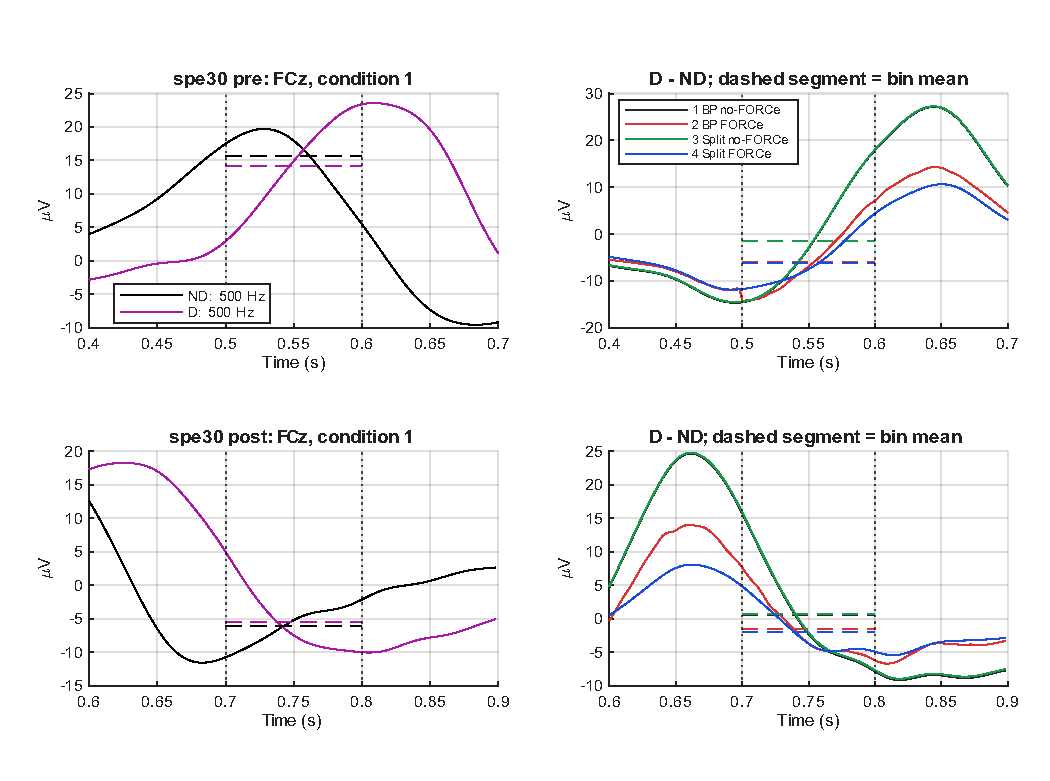
\includegraphics[width=\linewidth,height=.64\textheight,keepaspectratio]{figures/bin_cancellation_examples.pdf}
\caption{Left: original condition-1 ND/D means, with dashed horizontal bin means. Right: original D--ND means across all four processing conditions and their bin means. Dotted boundaries delimit the selected bin: 0.5--0.6 s pre and 0.7--0.8 s post. This is an illustration of representation loss, not proof of reduced decoding accuracy.}\end{figure}
\clearpage\section{Feature plots by participant and session}\label{app:features}
\subsection*{mle01 / pre: Original sample means and bin means}
Matched trials: ND $n=309$, D $n=166$ in every processing condition.
\begin{figure}[H]\centering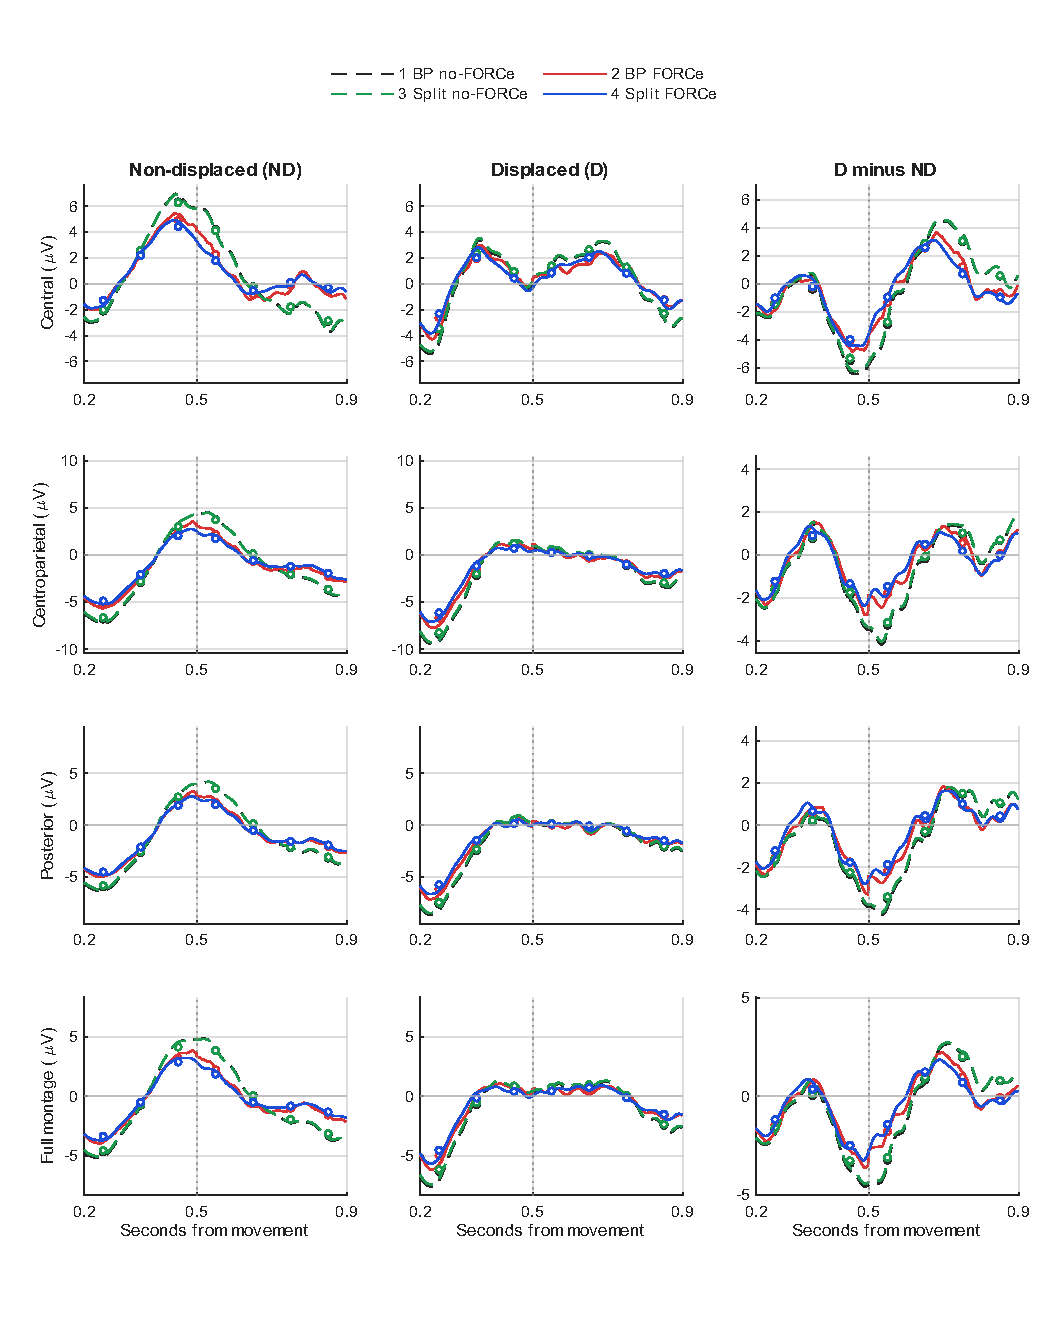
\includegraphics[width=\linewidth,height=.76\textheight,keepaspectratio]{figures/mle01_pre_means.pdf}\caption{Lines show original 500 Hz trial means; circles show 100 ms means at bin centres, with no interpolation between them. Rows illustrate the mean across channels in each named set; channels remain separate in the actual vectors. ND/D share a row scale, with a separate difference scale. No-FORCe is dashed, FORCe solid; the dotted line marks the +0.5 s join.}\end{figure}
\clearpage
\subsection*{mle01 / pre: Individual channel-feature separation}
Matched trials: ND $n=309$, D $n=166$ in every processing condition.
\begin{figure}[H]\centering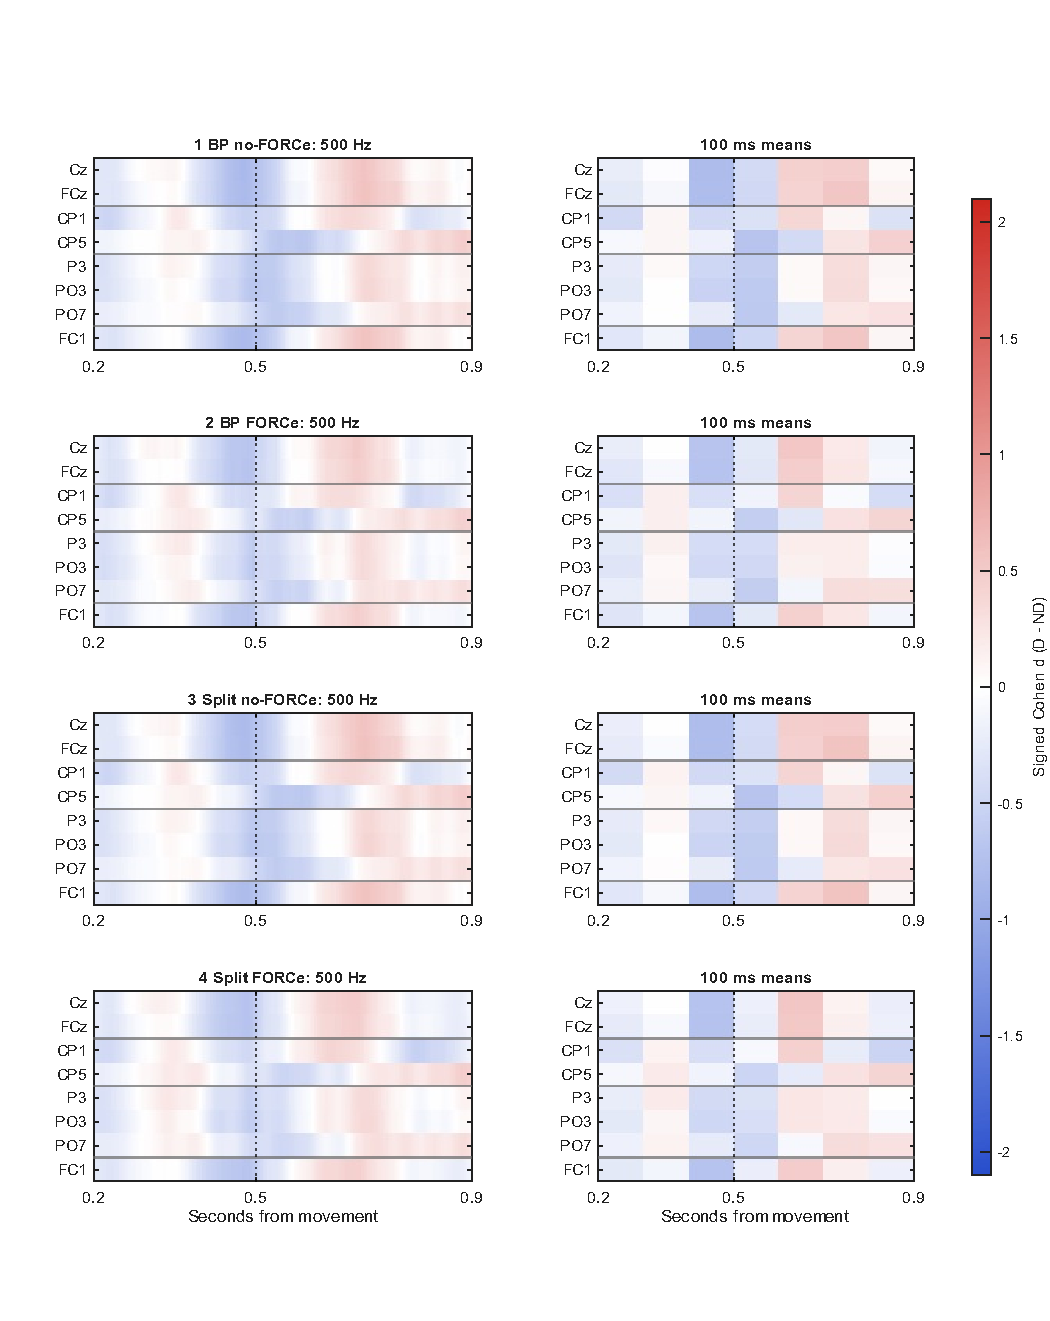
\includegraphics[width=\linewidth,height=.76\textheight,keepaspectratio]{figures/mle01_pre_separation.pdf}\caption{Signed Cohen $d$ for each original time point (left) and each 100 ms scalar feature (right). Blue means D below ND; red means D above ND. All panels in the report share limits $\pm2.1$. Horizontal divisions identify Central, Centroparietal, Posterior and FC1 (included only in Full). The bin effect uses the variance of bin means, so it is not an average of the pointwise effects. These are descriptive maps, not significance or classifier-performance maps.}\end{figure}
\clearpage
\subsection*{mle01 / post: Original sample means and bin means}
Matched trials: ND $n=218$, D $n=114$ in every processing condition.
\begin{figure}[H]\centering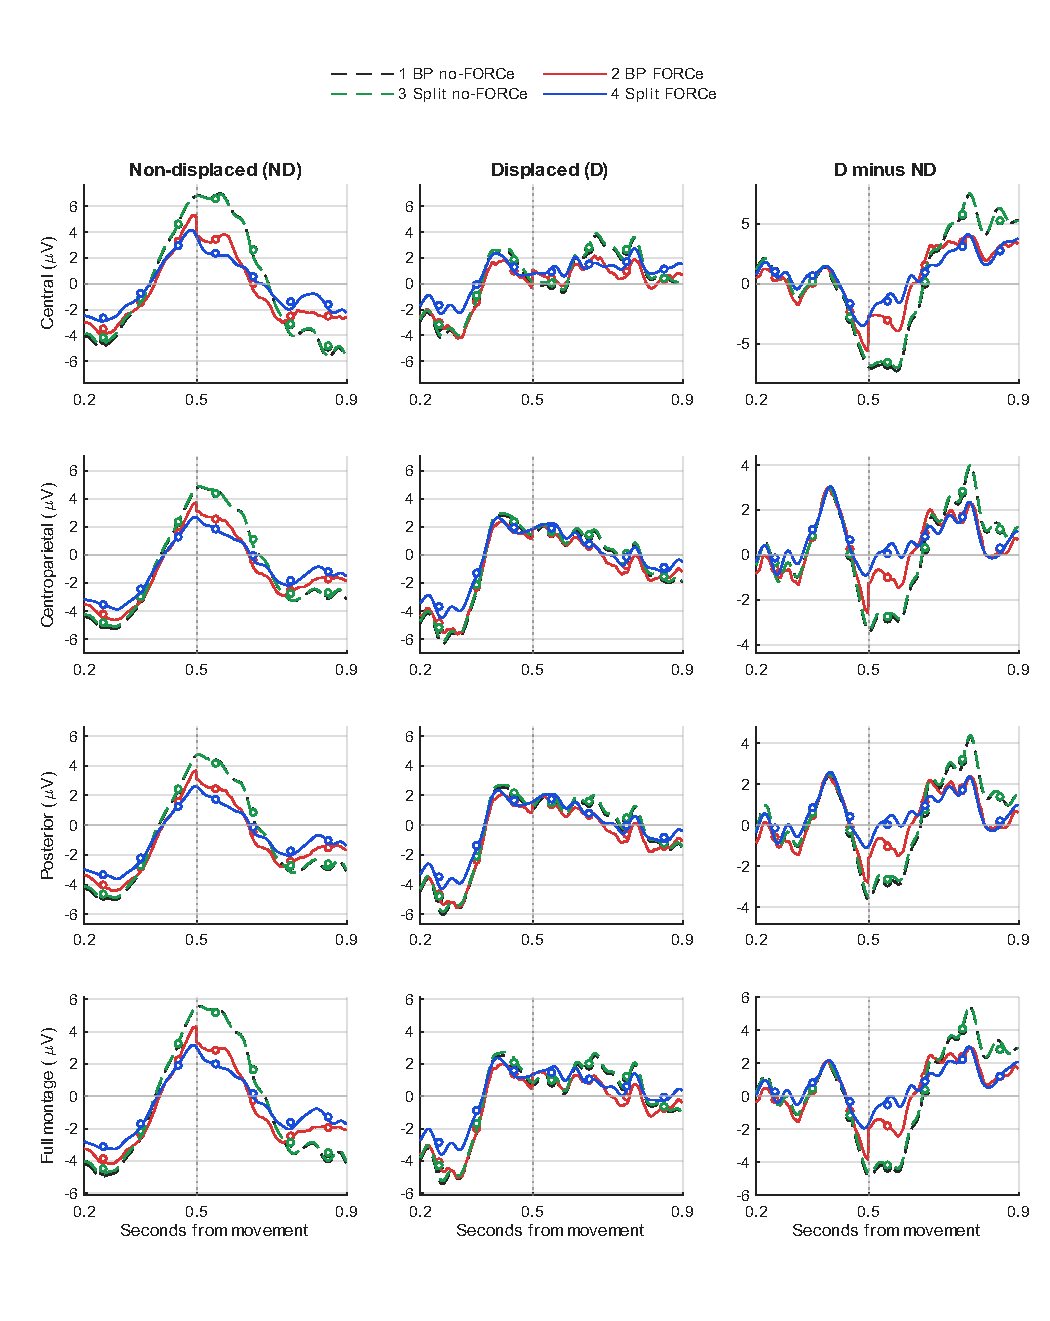
\includegraphics[width=\linewidth,height=.76\textheight,keepaspectratio]{figures/mle01_post_means.pdf}\caption{Lines show original 500 Hz trial means; circles show 100 ms means at bin centres, with no interpolation between them. Rows illustrate the mean across channels in each named set; channels remain separate in the actual vectors. ND/D share a row scale, with a separate difference scale. No-FORCe is dashed, FORCe solid; the dotted line marks the +0.5 s join.}\end{figure}
\clearpage
\subsection*{mle01 / post: Individual channel-feature separation}
Matched trials: ND $n=218$, D $n=114$ in every processing condition.
\begin{figure}[H]\centering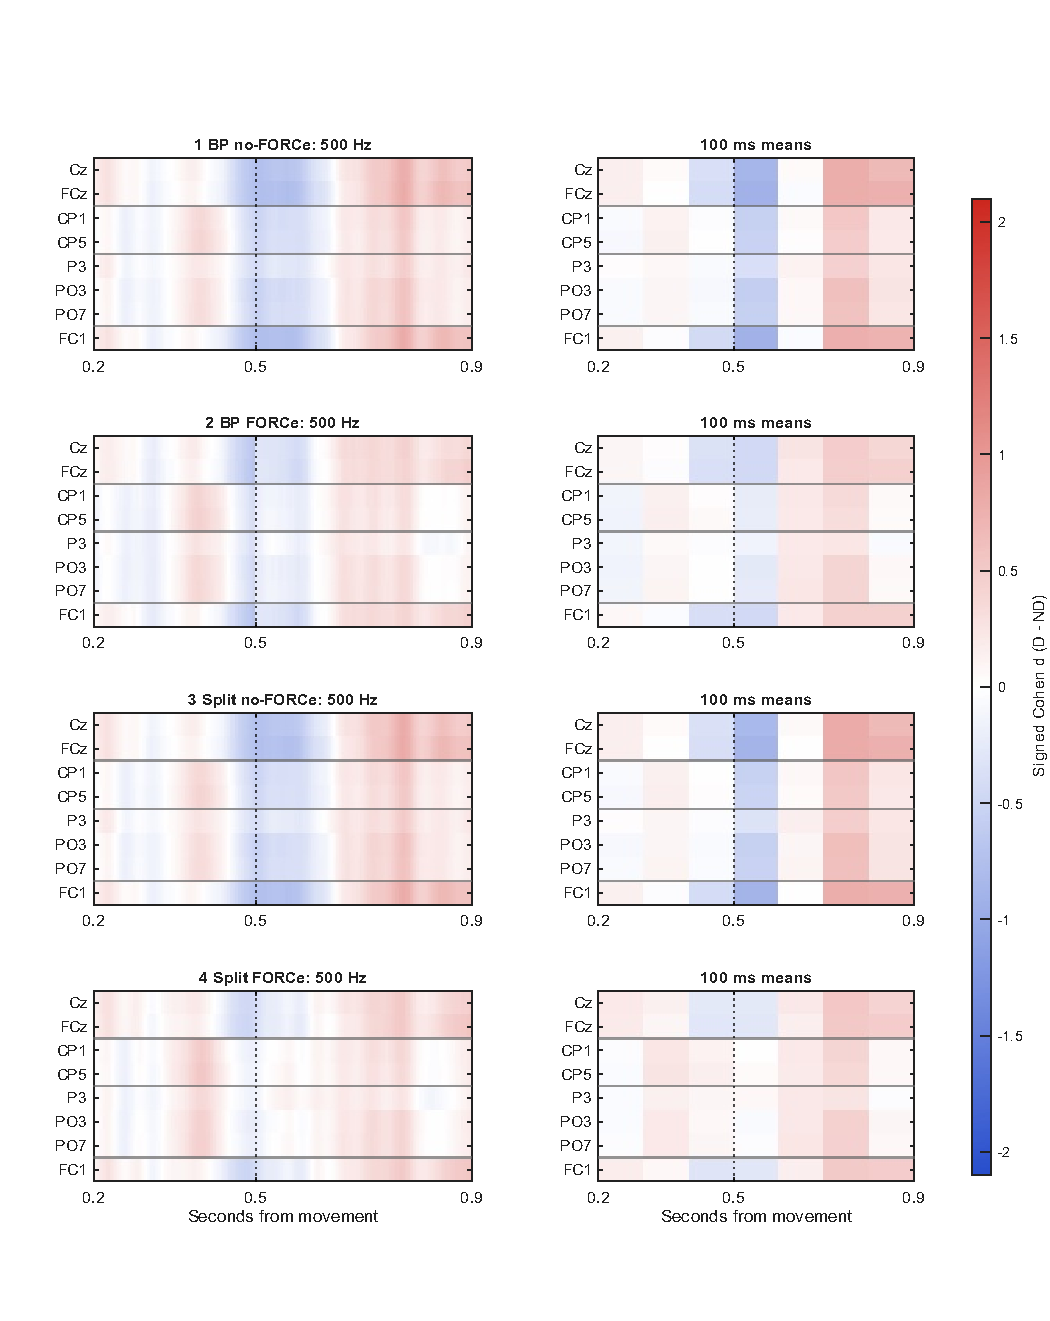
\includegraphics[width=\linewidth,height=.76\textheight,keepaspectratio]{figures/mle01_post_separation.pdf}\caption{Signed Cohen $d$ for each original time point (left) and each 100 ms scalar feature (right). Blue means D below ND; red means D above ND. All panels in the report share limits $\pm2.1$. Horizontal divisions identify Central, Centroparietal, Posterior and FC1 (included only in Full). The bin effect uses the variance of bin means, so it is not an average of the pointwise effects. These are descriptive maps, not significance or classifier-performance maps.}\end{figure}
\clearpage
\subsection*{mle01 / retest: Original sample means and bin means}
Matched trials: ND $n=237$, D $n=132$ in every processing condition.
\begin{figure}[H]\centering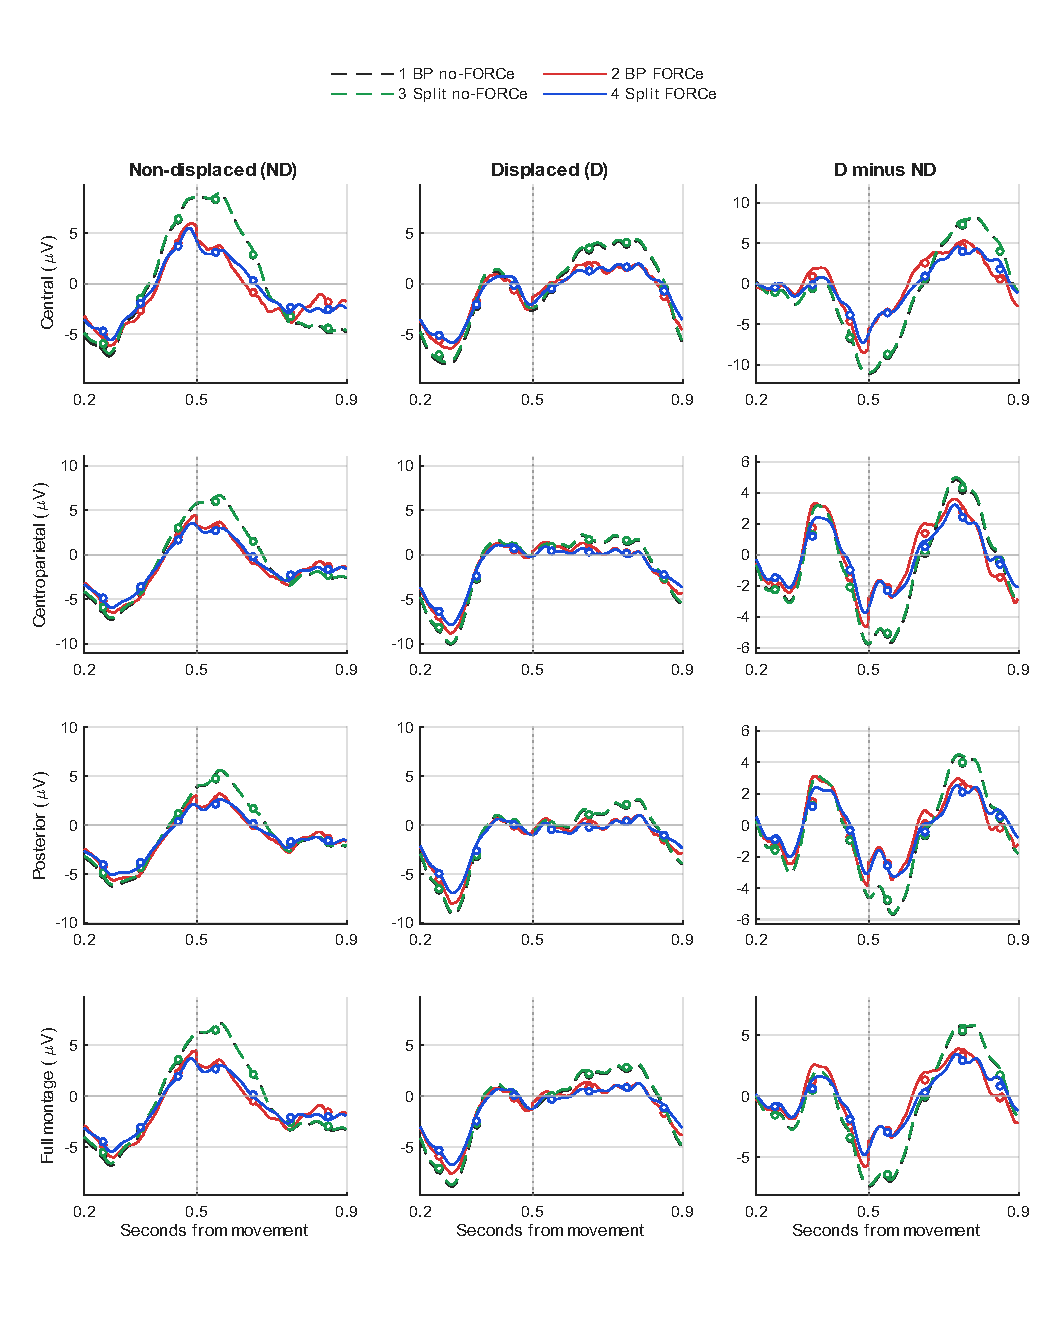
\includegraphics[width=\linewidth,height=.76\textheight,keepaspectratio]{figures/mle01_retest_means.pdf}\caption{Lines show original 500 Hz trial means; circles show 100 ms means at bin centres, with no interpolation between them. Rows illustrate the mean across channels in each named set; channels remain separate in the actual vectors. ND/D share a row scale, with a separate difference scale. No-FORCe is dashed, FORCe solid; the dotted line marks the +0.5 s join.}\end{figure}
\clearpage
\subsection*{mle01 / retest: Individual channel-feature separation}
Matched trials: ND $n=237$, D $n=132$ in every processing condition.
\begin{figure}[H]\centering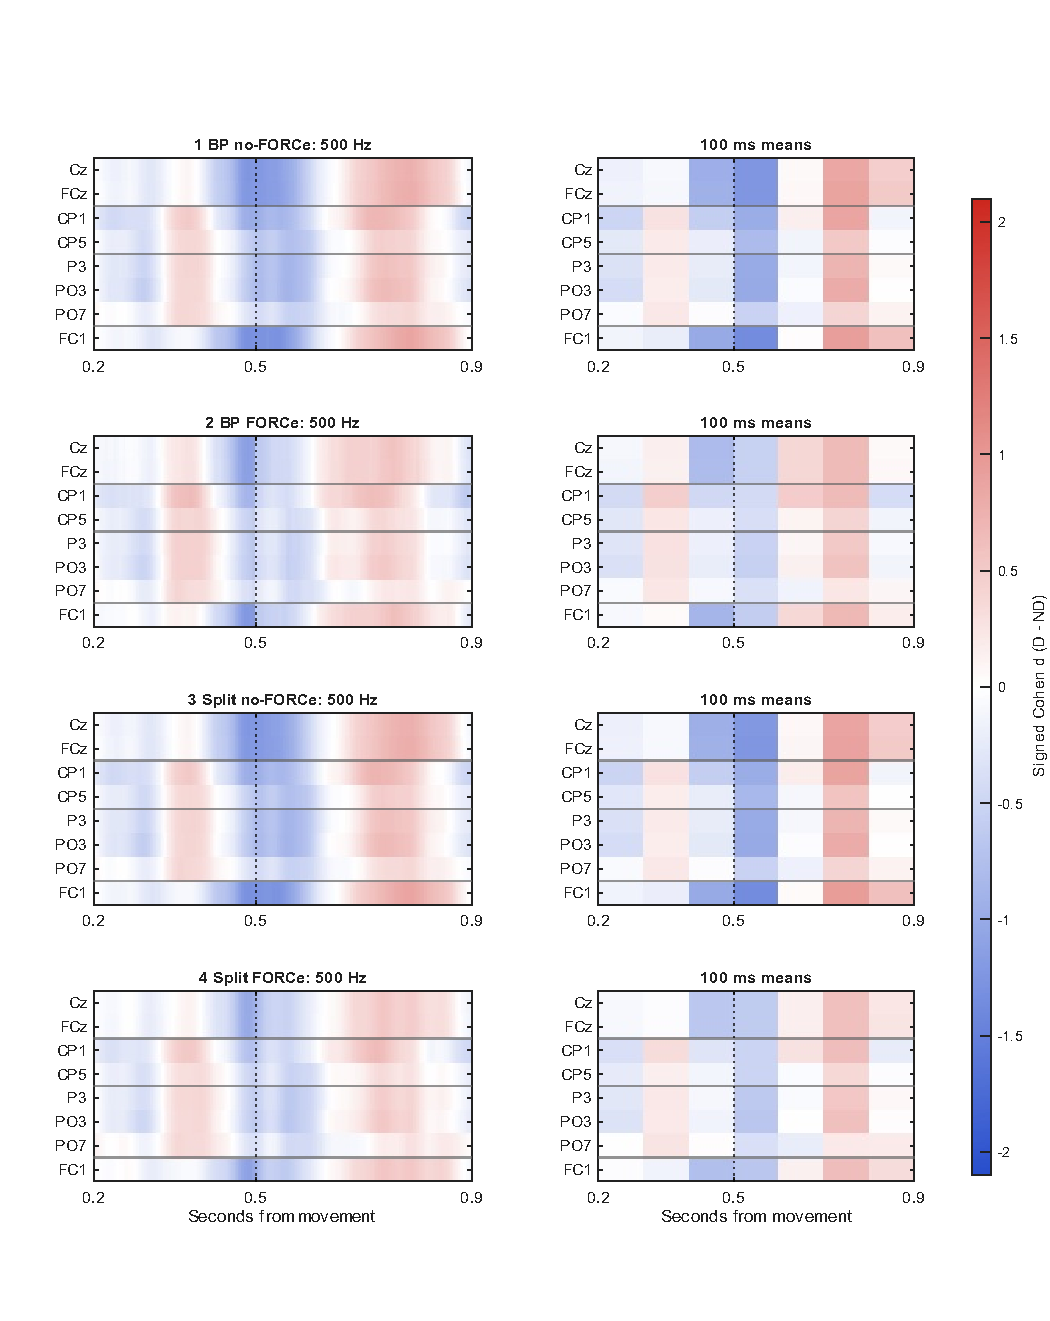
\includegraphics[width=\linewidth,height=.76\textheight,keepaspectratio]{figures/mle01_retest_separation.pdf}\caption{Signed Cohen $d$ for each original time point (left) and each 100 ms scalar feature (right). Blue means D below ND; red means D above ND. All panels in the report share limits $\pm2.1$. Horizontal divisions identify Central, Centroparietal, Posterior and FC1 (included only in Full). The bin effect uses the variance of bin means, so it is not an average of the pointwise effects. These are descriptive maps, not significance or classifier-performance maps.}\end{figure}
\clearpage
\subsection*{spe30 / pre: Original sample means and bin means}
Matched trials: ND $n=326$, D $n=169$ in every processing condition.
\begin{figure}[H]\centering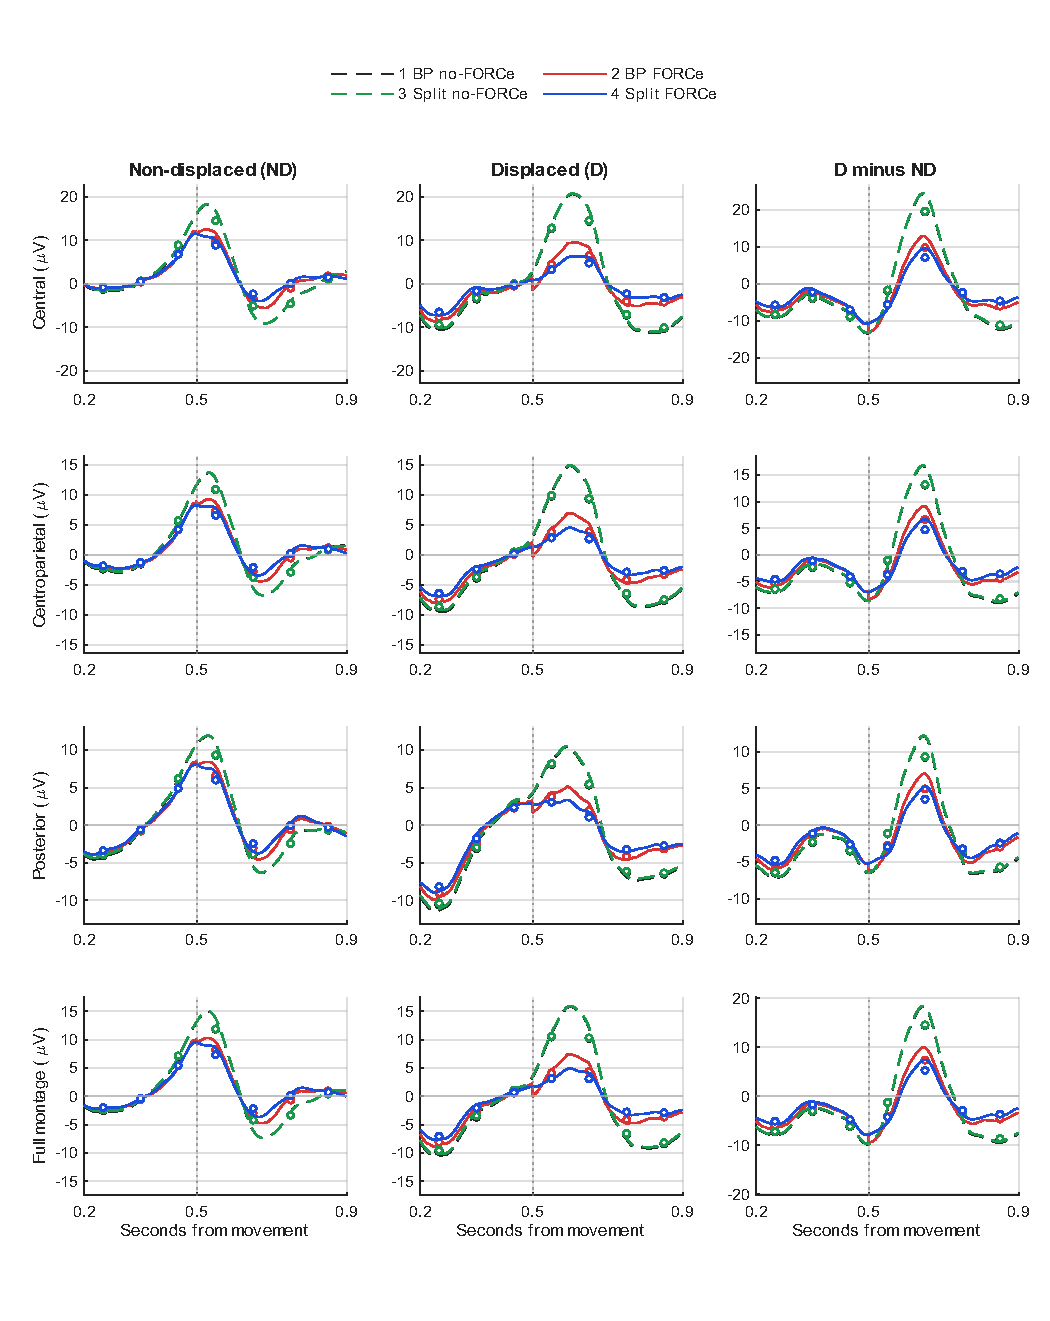
\includegraphics[width=\linewidth,height=.76\textheight,keepaspectratio]{figures/spe30_pre_means.pdf}\caption{Lines show original 500 Hz trial means; circles show 100 ms means at bin centres, with no interpolation between them. Rows illustrate the mean across channels in each named set; channels remain separate in the actual vectors. ND/D share a row scale, with a separate difference scale. No-FORCe is dashed, FORCe solid; the dotted line marks the +0.5 s join.}\end{figure}
\clearpage
\subsection*{spe30 / pre: Individual channel-feature separation}
Matched trials: ND $n=326$, D $n=169$ in every processing condition.
\begin{figure}[H]\centering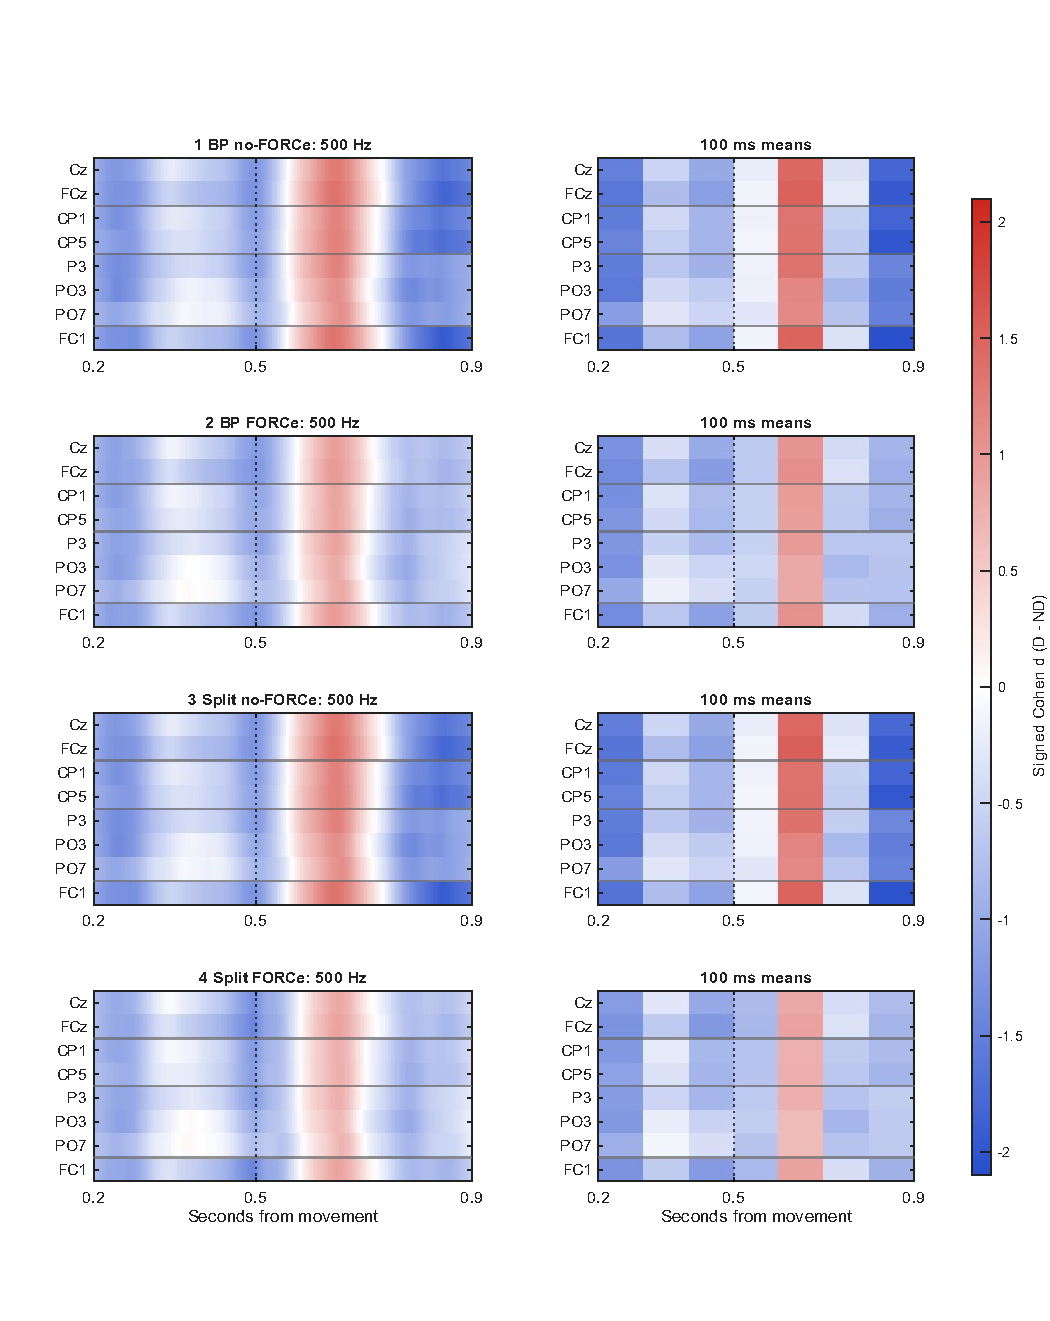
\includegraphics[width=\linewidth,height=.76\textheight,keepaspectratio]{figures/spe30_pre_separation.pdf}\caption{Signed Cohen $d$ for each original time point (left) and each 100 ms scalar feature (right). Blue means D below ND; red means D above ND. All panels in the report share limits $\pm2.1$. Horizontal divisions identify Central, Centroparietal, Posterior and FC1 (included only in Full). The bin effect uses the variance of bin means, so it is not an average of the pointwise effects. These are descriptive maps, not significance or classifier-performance maps.}\end{figure}
\clearpage
\subsection*{spe30 / post: Original sample means and bin means}
Matched trials: ND $n=329$, D $n=169$ in every processing condition.
\begin{figure}[H]\centering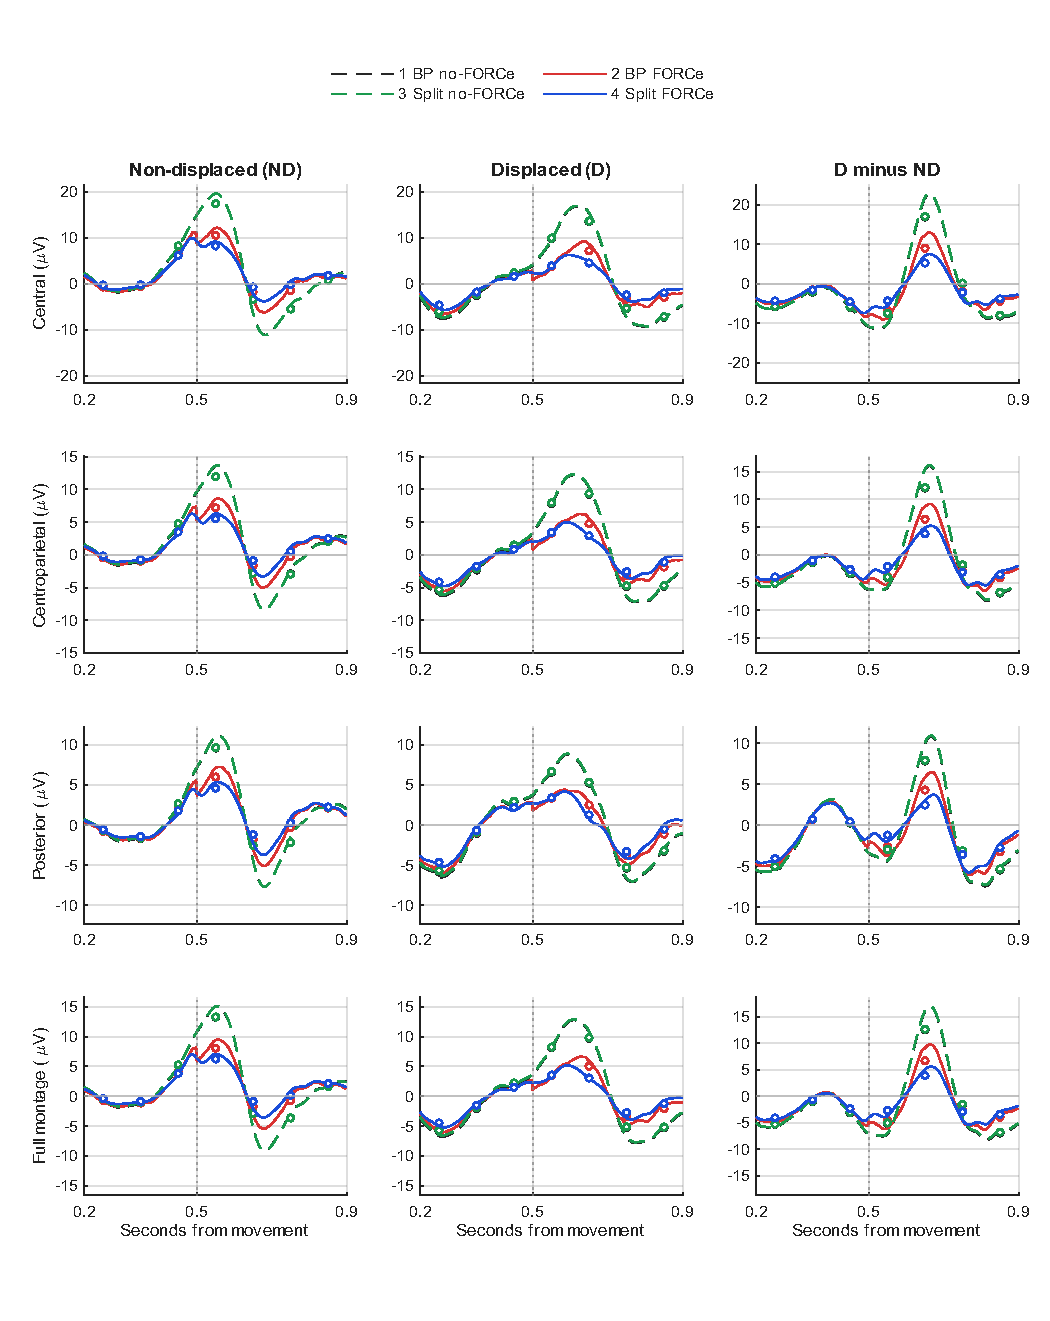
\includegraphics[width=\linewidth,height=.76\textheight,keepaspectratio]{figures/spe30_post_means.pdf}\caption{Lines show original 500 Hz trial means; circles show 100 ms means at bin centres, with no interpolation between them. Rows illustrate the mean across channels in each named set; channels remain separate in the actual vectors. ND/D share a row scale, with a separate difference scale. No-FORCe is dashed, FORCe solid; the dotted line marks the +0.5 s join.}\end{figure}
\clearpage
\subsection*{spe30 / post: Individual channel-feature separation}
Matched trials: ND $n=329$, D $n=169$ in every processing condition.
\begin{figure}[H]\centering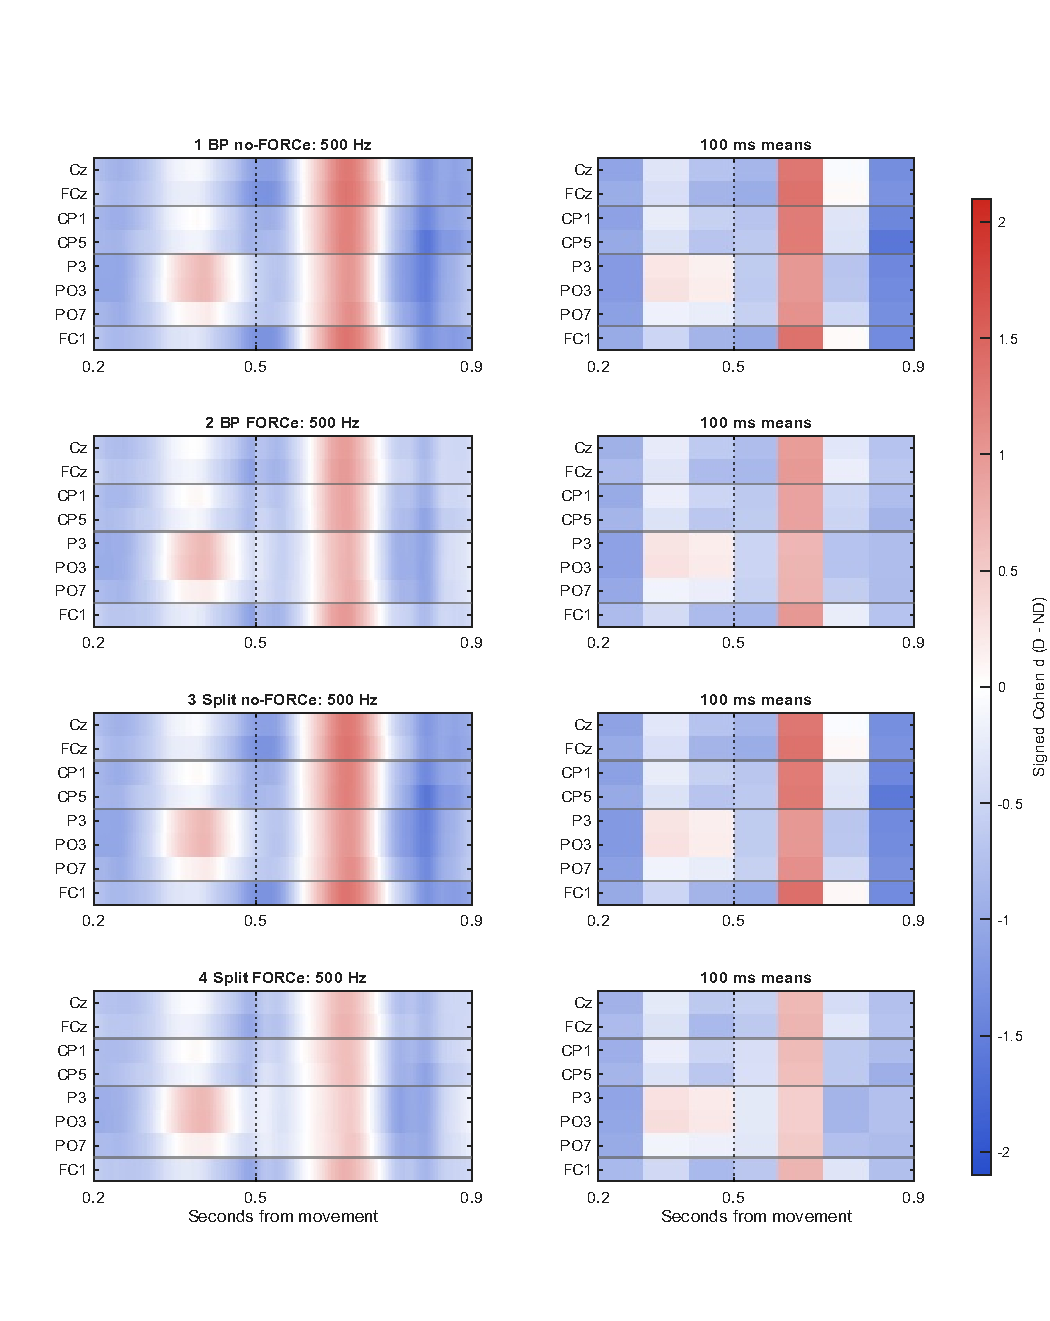
\includegraphics[width=\linewidth,height=.76\textheight,keepaspectratio]{figures/spe30_post_separation.pdf}\caption{Signed Cohen $d$ for each original time point (left) and each 100 ms scalar feature (right). Blue means D below ND; red means D above ND. All panels in the report share limits $\pm2.1$. Horizontal divisions identify Central, Centroparietal, Posterior and FC1 (included only in Full). The bin effect uses the variance of bin means, so it is not an average of the pointwise effects. These are descriptive maps, not significance or classifier-performance maps.}\end{figure}
\clearpage
\subsection*{spe30 / retest: Original sample means and bin means}
Matched trials: ND $n=260$, D $n=133$ in every processing condition.
\begin{figure}[H]\centering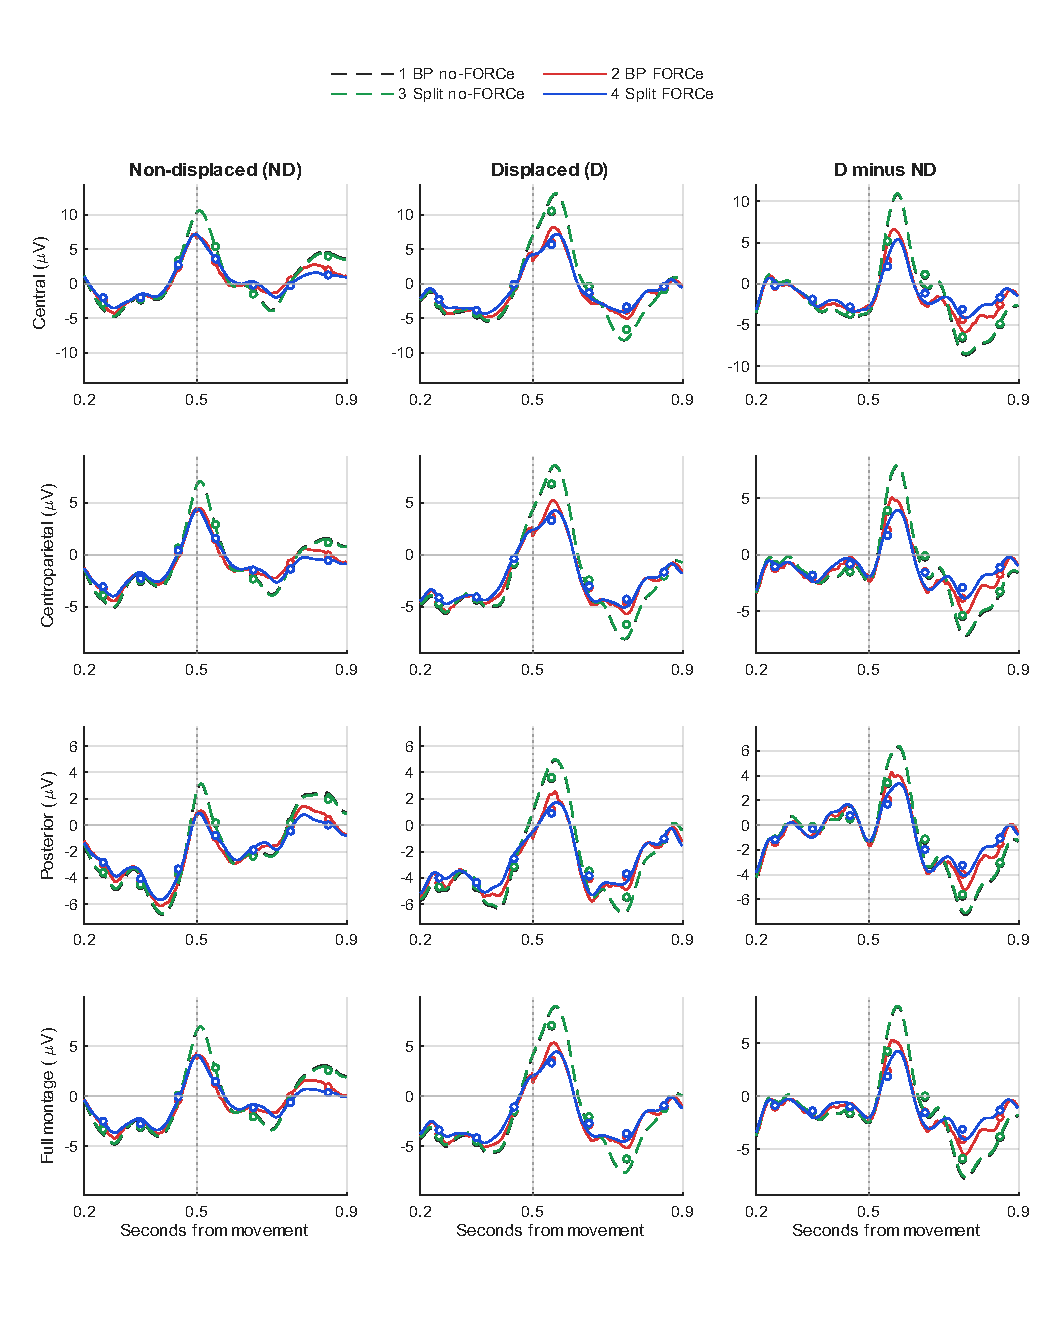
\includegraphics[width=\linewidth,height=.76\textheight,keepaspectratio]{figures/spe30_retest_means.pdf}\caption{Lines show original 500 Hz trial means; circles show 100 ms means at bin centres, with no interpolation between them. Rows illustrate the mean across channels in each named set; channels remain separate in the actual vectors. ND/D share a row scale, with a separate difference scale. No-FORCe is dashed, FORCe solid; the dotted line marks the +0.5 s join.}\end{figure}
\clearpage
\subsection*{spe30 / retest: Individual channel-feature separation}
Matched trials: ND $n=260$, D $n=133$ in every processing condition.
\begin{figure}[H]\centering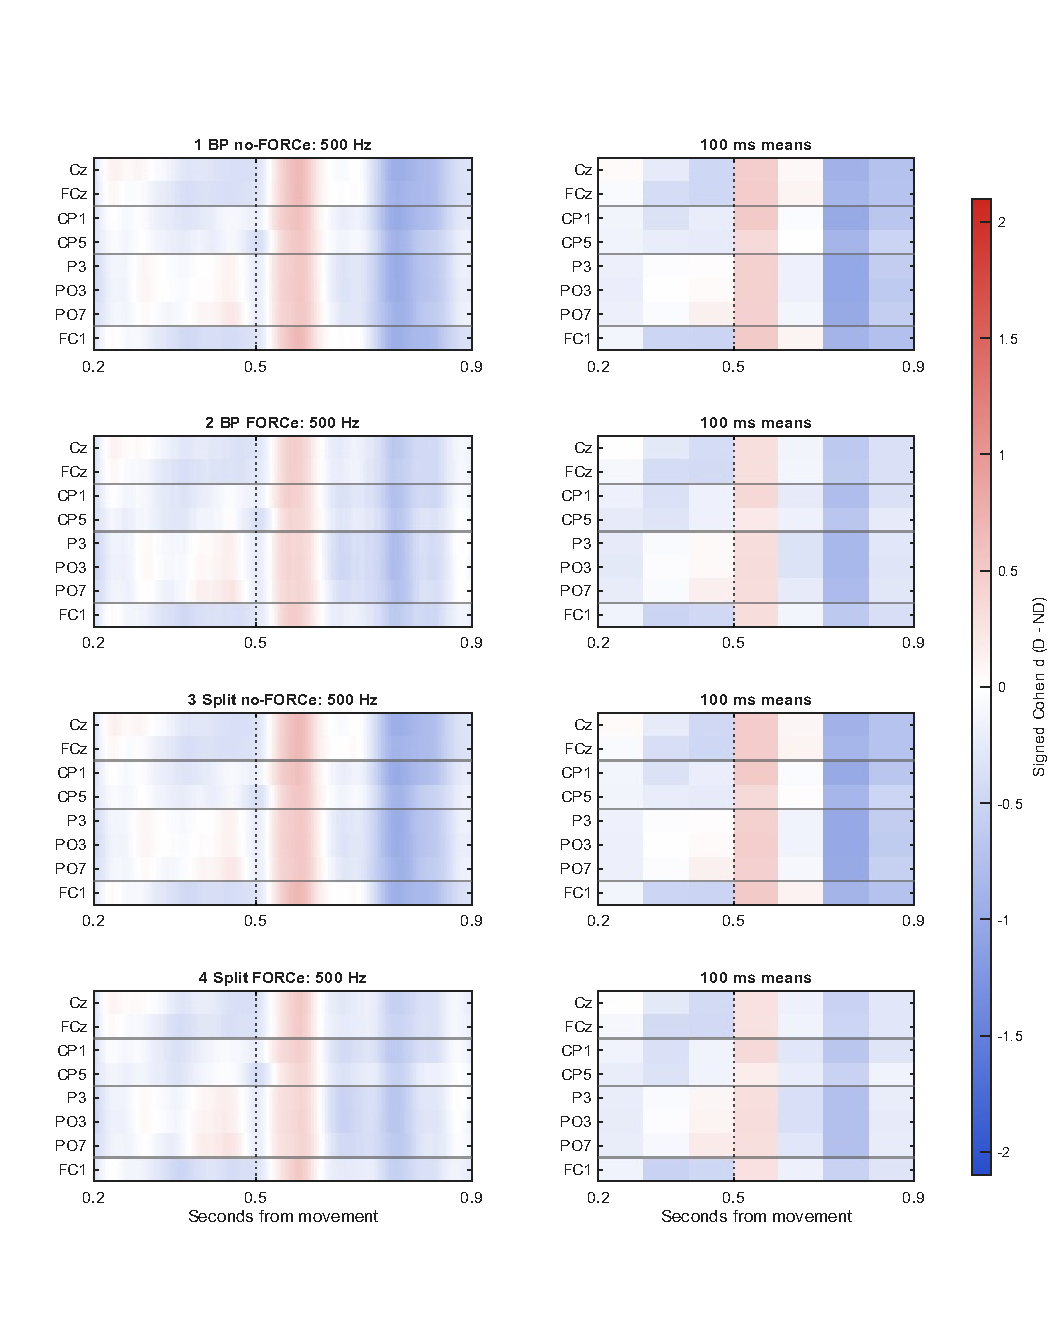
\includegraphics[width=\linewidth,height=.76\textheight,keepaspectratio]{figures/spe30_retest_separation.pdf}\caption{Signed Cohen $d$ for each original time point (left) and each 100 ms scalar feature (right). Blue means D below ND; red means D above ND. All panels in the report share limits $\pm2.1$. Horizontal divisions identify Central, Centroparietal, Posterior and FC1 (included only in Full). The bin effect uses the variance of bin means, so it is not an average of the pointwise effects. These are descriptive maps, not significance or classifier-performance maps.}\end{figure}
\clearpage\section{Repeatability by participant, session and channel set}\label{app:repeat}
\subsection*{mle01: Independent balanced trial halves}
Original-sample waveforms over $[0.2,0.9)$ s. All four processing conditions use matched IDs.
\begin{figure}[H]\centering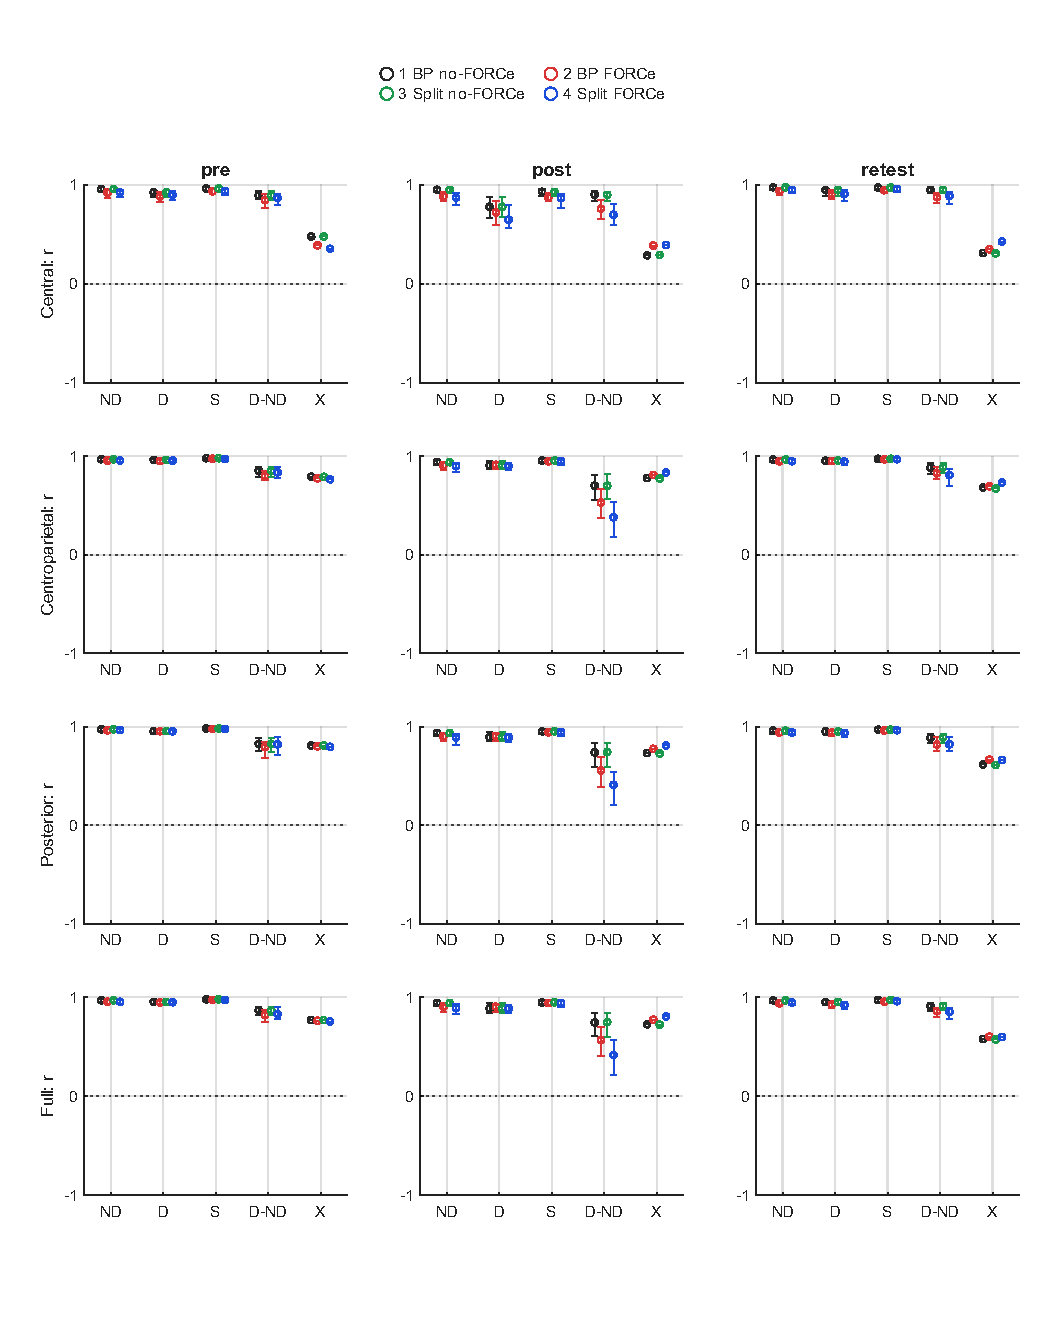
\includegraphics[width=\linewidth,height=.76\textheight,keepaspectratio]{figures/mle01_balanced_split_half.pdf}\caption{Each marker is a channel-median correlation, then median over 50 stratified disjoint-half comparisons. Whiskers are 10th--90th percentiles over repeats, not confidence intervals. ND/D are same-class agreement; S is the equally weighted shared response; D--ND is the difference; X averages the two directional cross-class correlation summaries and is shown without whiskers.}\end{figure}
\clearpage
\subsection*{mle01: Distinct runs within sessions}
Original-sample waveforms over $[0.2,0.9)$ s. All four processing conditions use matched IDs.
\begin{figure}[H]\centering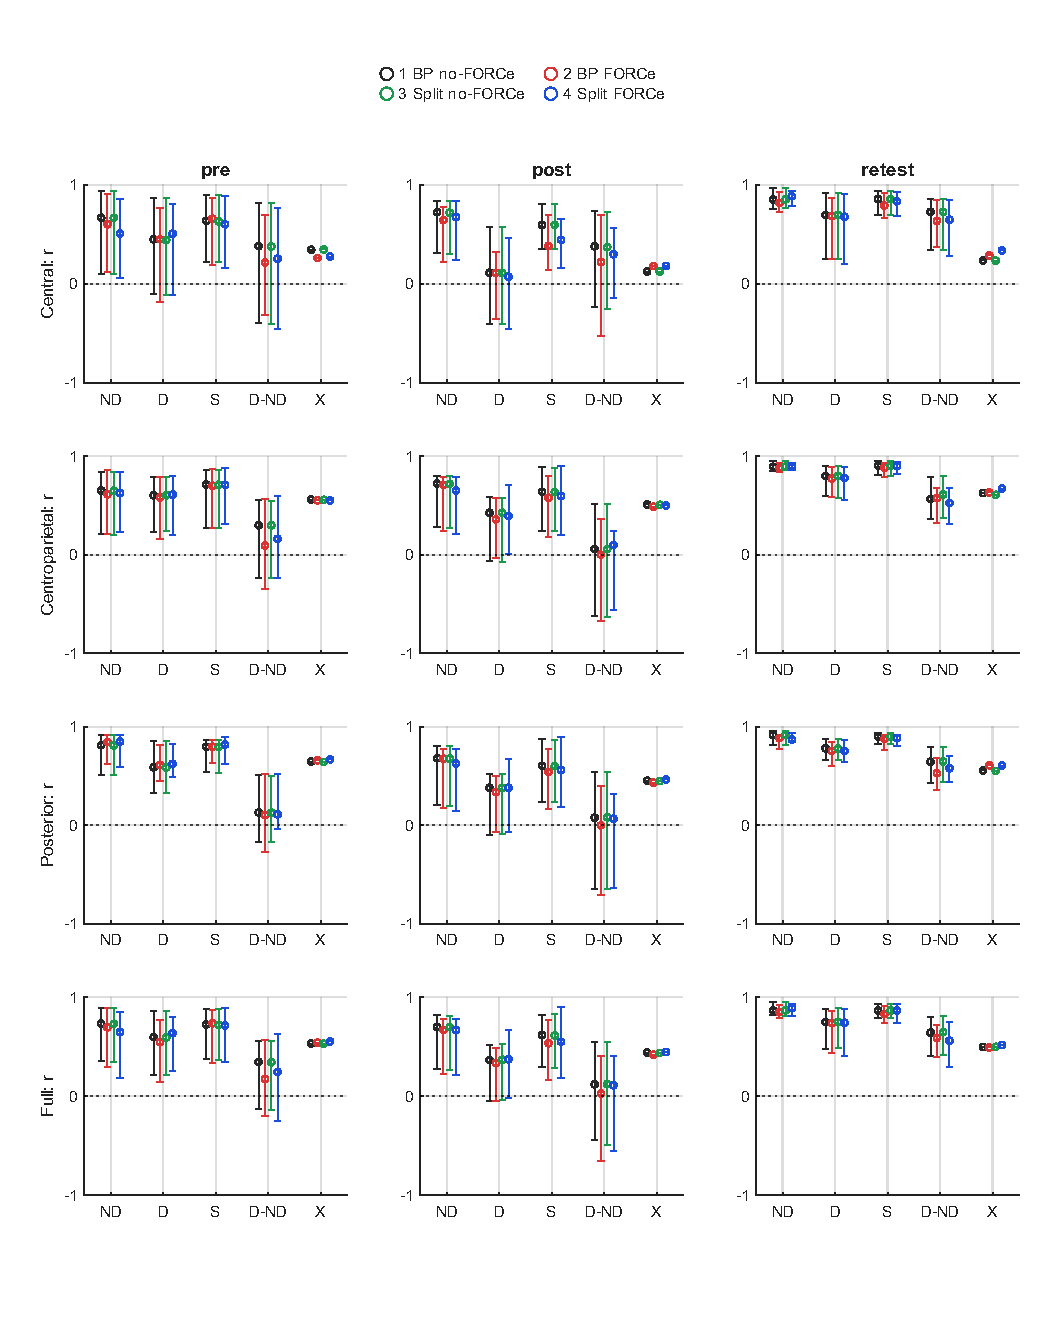
\includegraphics[width=\linewidth,height=.76\textheight,keepaspectratio]{figures/mle01_between_runs.pdf}\caption{Each marker is the median over run pairs of the channel-median correlation. Whiskers are the 10th--90th percentiles over pairs, not confidence intervals. Pairs share runs; per-run averaging counts are smaller than pooled split halves. ND/D are same-class agreement; S is the equally weighted shared response; D--ND is the difference; X averages the two directional cross-class correlation summaries and is shown without whiskers.}\end{figure}
\clearpage
\subsection*{mle01: Full session-average comparison}
Original-sample waveforms over $[0.2,0.9)$ s. All four processing conditions use matched IDs.
\begin{figure}[H]\centering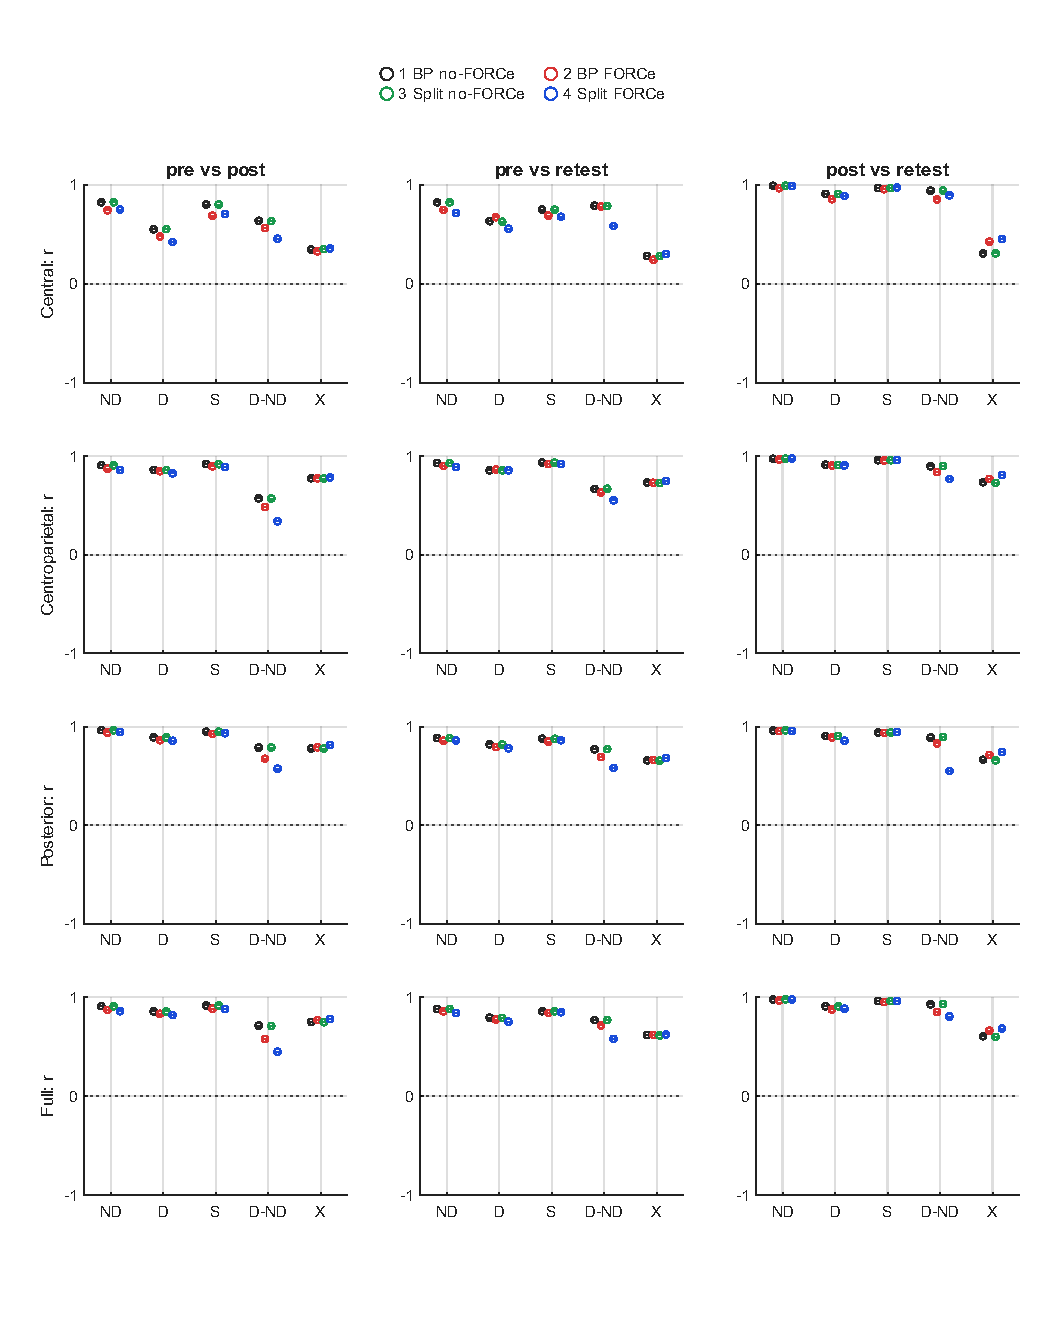
\includegraphics[width=\linewidth,height=.76\textheight,keepaspectratio]{figures/mle01_between_sessions.pdf}\caption{Each marker is the channel-median correlation between the two full session means. There is one comparison per set/waveform/condition, so there are no variability whiskers. ND/D are same-class agreement; S is the equally weighted shared response; D--ND is the difference; X averages the two directional cross-class correlation summaries and is shown without whiskers.}\end{figure}
\clearpage
\subsection*{spe30: Independent balanced trial halves}
Original-sample waveforms over $[0.2,0.9)$ s. All four processing conditions use matched IDs.
\begin{figure}[H]\centering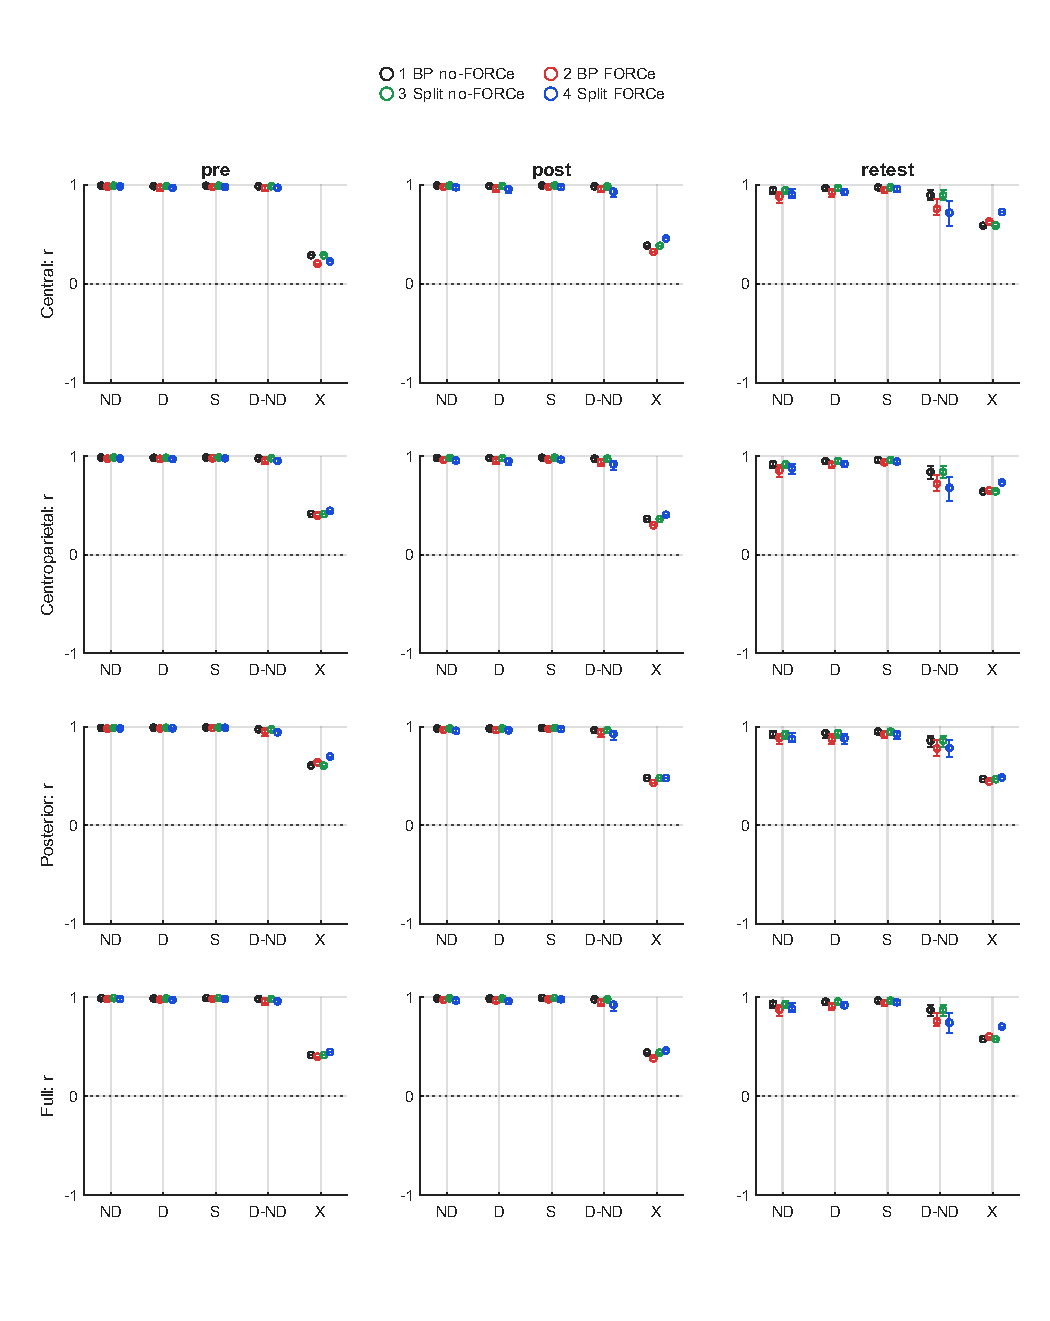
\includegraphics[width=\linewidth,height=.76\textheight,keepaspectratio]{figures/spe30_balanced_split_half.pdf}\caption{Each marker is a channel-median correlation, then median over 50 stratified disjoint-half comparisons. Whiskers are 10th--90th percentiles over repeats, not confidence intervals. ND/D are same-class agreement; S is the equally weighted shared response; D--ND is the difference; X averages the two directional cross-class correlation summaries and is shown without whiskers.}\end{figure}
\clearpage
\subsection*{spe30: Distinct runs within sessions}
Original-sample waveforms over $[0.2,0.9)$ s. All four processing conditions use matched IDs.
\begin{figure}[H]\centering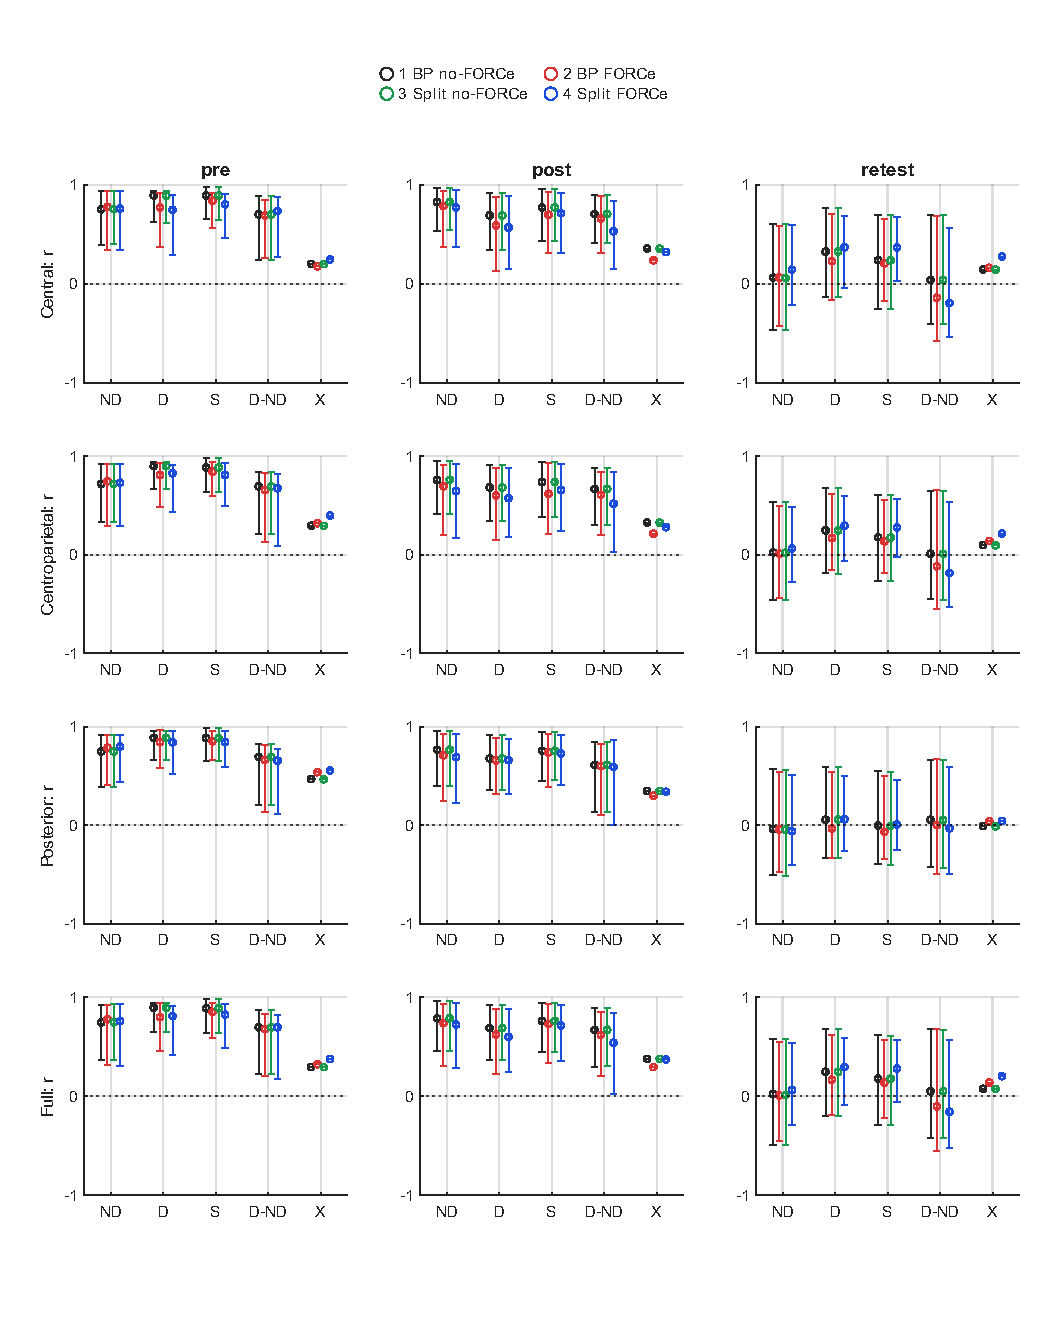
\includegraphics[width=\linewidth,height=.76\textheight,keepaspectratio]{figures/spe30_between_runs.pdf}\caption{Each marker is the median over run pairs of the channel-median correlation. Whiskers are the 10th--90th percentiles over pairs, not confidence intervals. Pairs share runs; per-run averaging counts are smaller than pooled split halves. ND/D are same-class agreement; S is the equally weighted shared response; D--ND is the difference; X averages the two directional cross-class correlation summaries and is shown without whiskers.}\end{figure}
\clearpage
\subsection*{spe30: Full session-average comparison}
Original-sample waveforms over $[0.2,0.9)$ s. All four processing conditions use matched IDs.
\begin{figure}[H]\centering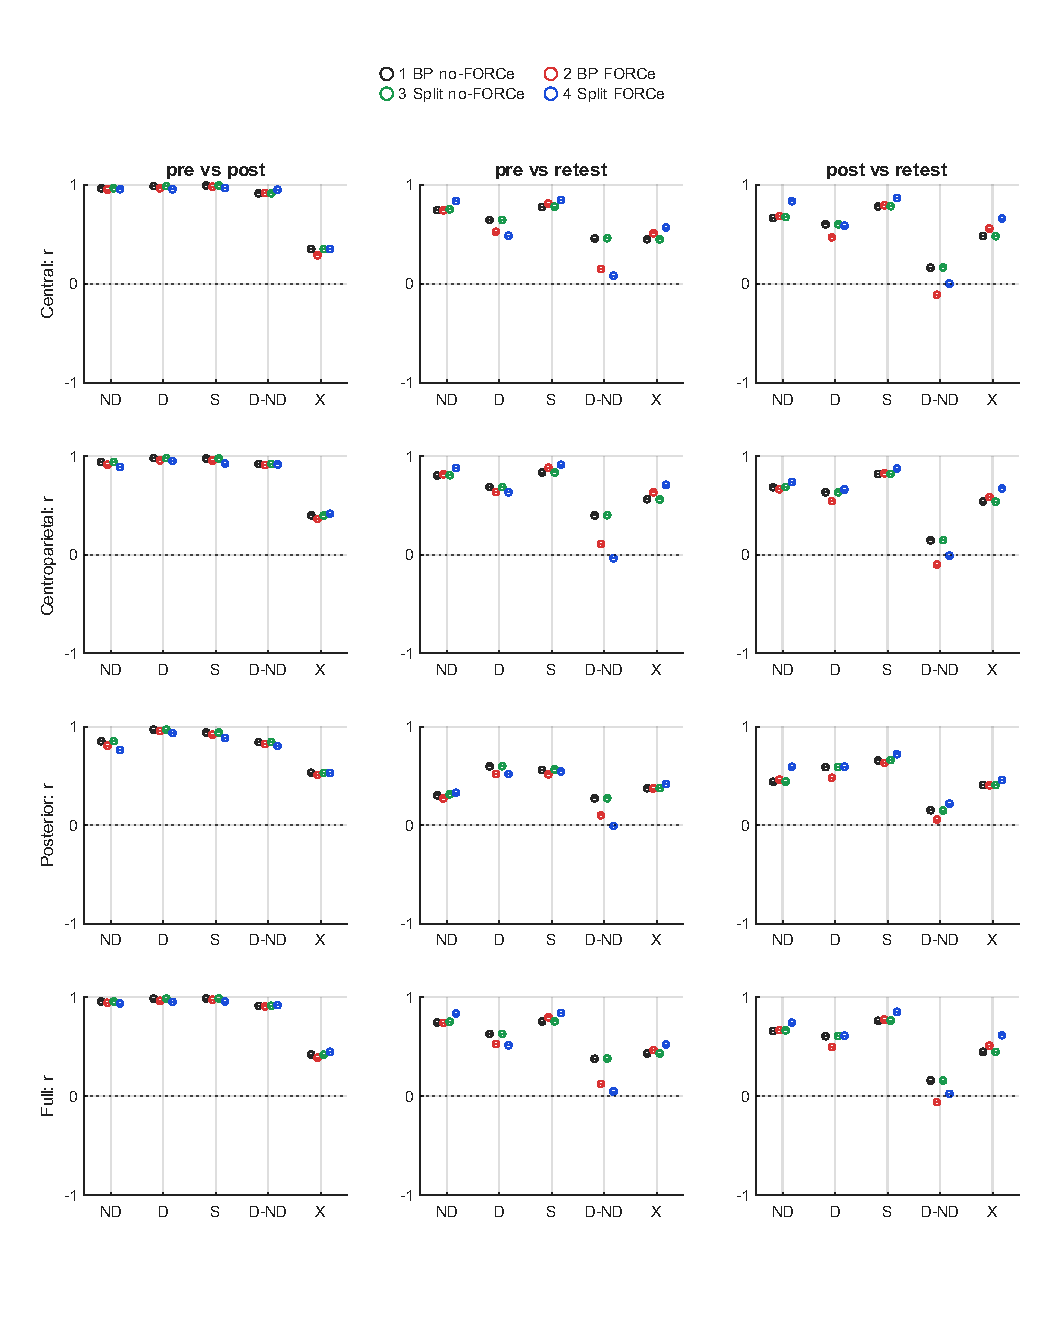
\includegraphics[width=\linewidth,height=.76\textheight,keepaspectratio]{figures/spe30_between_sessions.pdf}\caption{Each marker is the channel-median correlation between the two full session means. There is one comparison per set/waveform/condition, so there are no variability whiskers. ND/D are same-class agreement; S is the equally weighted shared response; D--ND is the difference; X averages the two directional cross-class correlation summaries and is shown without whiskers.}\end{figure}
\end{document}
